\documentclass[
  BCOR12mm,
  letterpaper,
  11pt,
  headsepline,
  pointlessnumbers,
  tablecaptionabove,
  onelinecaption,
  headinclude,
  appendixprefix,
  idxtotoc,
  bibtotoc,
  twoside,
  titlepage
]{scrreprt}

\usepackage{UT}

% booktabs is for toprule, bottomrule, etc. in tables.
\usepackage{booktabs}
\usepackage{multirow}
\usepackage{array}   %stellt den Befehl \newcolumntype bereit
\usepackage{hyperref} % Links im dokument
%\usepackage[utf8]{inputenc} %unicode support

\hypersetup{
              bookmarks={true},
              bookmarksopen={true},
              bookmarksopenlevel={0},
              bookmarksnumbered={true},
              breaklinks={true},
              colorlinks={false},
              pdfpagemode={UseOutlines},
              pdftitle={YOUR SOFTWARE'S NAME},
              pdfauthor={YOUR NAME},
              pdfsubject={User's Guide},
              pdfkeywords={Key word 1} {Key word 1} {...} {Key word n}
              pdftex,
              pdffitwindow={true},
              pdfstartview={FitV},
              pdfnewwindow={false},
              pdfdisplaydoctitle={true},
              pdfhighlight={/P},
              plainpages={false},
              unicode={true},
              urlcolor={blue}
}

%HYPHENATION
\hyphenation{
}
%%%%%%%%%%%%%%%%%%%%%%%%%%%%%%%%%
% Gestaltung der Titelseite     %
%%%%%%%%%%%%%%%%%%%%%%%%%%%%%%%%%

\newcolumntype{C}[1]{>{\centering\arraybackslash}m{#1}}
\newcolumntype{L}[1]{>{\centering\arraybackslash}p{#1}}

\titlehead{\centering
\includegraphics[width=0.75\textwidth]{img/UT_WBMW_mathnat_4C}}
\subject{User's Guide}
\title{
\centering
\begin{tabular}{C{5cm}L{5cm}}
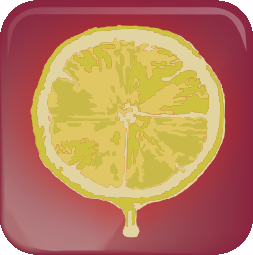
\includegraphics[width=.3\columnwidth]{img/LOGO.png} &
YOUR SOFTWARE'S NAME \\
\end{tabular}
}
\subtitle{Interesting sub title}


\author{Your Name\thanks{Corresponding author:
\href{mailto:your.name@uni-tuebingen.de}{your.name@uni-tuebingen.de}}\and
Second Author\and Third Author}
\date{\today}
\publishers{Center for Bioinformatics Tuebingen (ZBIT)}



%%%%%%%%%%%%%%%%%%%%%%%%%%%%%%%%%
% Beginn des Dokumentes         %
%%%%%%%%%%%%%%%%%%%%%%%%%%%%%%%%%

\begin{document}


%%%%%%%%%%%%%%%%%%%%%%%%%%%%%%%%%
% Titelei                       %
%%%%%%%%%%%%%%%%%%%%%%%%%%%%%%%%%

\pagenumbering{roman}		% kleine lateinische Seitenzahlen
\maketitle
\begin{abstract}
The tool SBMLsqueezer facilitates the task of assigning kinetic equations to
reactions within biochemical network models in SBML format.
It analyzes each reaction of interest, selects applicable equations, and derives
appropriate units of all parameters contained in these equations.
If possible, components that SBMLsqueezer adds to your model are annotated with
\ac{SBO} and \ac{MIRIAM} tags.
Besides \emph{de-novo} creation of rate equations, SBMLsqueezer also offers
online access to the reaction kinetics database \ac{SABIO-RK}, where you can extract
experimentally determined rate laws for your model.
In both modes (\emph{de-novo} creation and database lookup), you can assign kinetic equations to all reactions of the model in
one single step, or select individual reactions of interest. 
Several settings allow you to customize the behavior of the program.
In particular, all choices made by SBMLsqueezer can be changed or influenced.
The program can be used in multiple ways: as a plug-in for the programm
CellDesigner, as a gadget for Garuda, as a stand-alone tool via its graphical
user interface, or as a command-line based tool.
Furthermore, the application programming interface allows you to integrate
SBMLsqueezer as an equation generating core into your end-user application.
An export function based on the integrated tool \SBMLLaTeXs{} allows you to
generate an exhaustive model report for scientific writing or further
processing.

\end{abstract}

\setcounter{tocdepth}{1}
\tableofcontents		% Inhaltsverzeichnis
% \listoffigures
% \listoftables

\cleardoublepage		% Erzeugt neue Leerseite. Muss ggf. auskommentiert werden.
\pagenumbering{arabic}		% Ab hier mit arabischen Zahlen numerieren


%%%%%%%%%%%%%%%%%%%%%%%%%%%%%%%%%
% Beginn der eigentlichen Arbeit%
%%%%%%%%%%%%%%%%%%%%%%%%%%%%%%%%%


\chapter{Introduction}

The program SBMLsqueezer is a versatile tool for the assembly and assignment of
complex kinetic equations of reactions and processes in biochemical networks
\citep{Draeger2008, Draeger2010a, Draeger2011a}.
The purpose of SBMLsqueezer is hence to assist you when creating kinetic equations for
a biochemical network, whose structure is already defined.
SBMLsqueezer can add missing information, such as undefined initial concentration values
or set some reacting species that represent genes to the boundary of the reaction system.
But its main purpose is the creation of rate laws, parameter objects, and their units.
The integrated \SBMLLaTeX can create an exhaustive model report that highlights all
model features.
A list of currently implemented rate laws that can be used for the \emph{de novo}
creation of kinetic laws can be found in \vref{chap:RateLaws}.

\section{Overview}

The data format understood by SBMLsqueezer is the
\SBML\footnote{Various information about \SBML can be found at \url{http://sbml.org}.}
in all of its levels and versions \citep{Hucka2001, Hucka2003, M.Hucka03012003, Hucka2007, Hucka2008,
Hucka2010a, Finney2003, Finney2006}.
When using \SBML Level~1 (not recommended), all generated equations are stored
in form of infix formula strings. For all other versions of \SBML, the generated
equations are stored in form of \MathML \citep{Buswell1999} expressions.

Kinetic equations contain a set of parameters, whose units must be derived to
ensure that the overall equation can be interpreted in units of the extent of the
respective reaction per time units.
To give an example for the most common scenario, you can assume that the units
of the rate law will simplify to a substance unit per time unit, for instance,
mole per second.
Other constellations, however, are possible, too.
When using SBMLsqueezer you do not have to care much about units because the
program does this for you.
Since Level~3, the \MathML subset understood by \SBML has been extended and also supports
units for actual numbers (integers or real values, which are not parameter values in this sense).
When using a model in this more recent format, SBMLsqueezer will also assign units
to numbers where necessary.

The program also annotates all created equations and parameters with appropriate
terms from the \SBO\footnote{For more information about \SBO see \url{http://www.ebi.ac.uk/sbo/main/}.}
(\acl{SBO}) and also
with \MIRIAM-compliant\footnote{The \MIRIAM registry is described at \url{http://co.mbine.org/standards/miriam}.}
controlled vocabulary terms (\acl{MIRIAM}), where appropriate \citep{Le2005, Novere2006b, Laible2007, Courtot2011}.

The selection of the kinetic equations is done automatically by the program,
where several settings allow users to influence the algorithm's choice.
In many cases, SBMLsqueezer suggests multiple equations for the same process,
from which the user can choose as desired.
This behavior of the program is important to ensure that only appropriate
equations can be selected at any time.

In order to decide, which equations can be applied to a reaction of interest,
SBMLsqueezer analyzes several properties, such as the number and type of
reactants, products, and modifiers, if the reaction is reversible, etc.
Here, reaction of interest means that the user can either select individual
reactions from a larger model and equip these with kinetic equations, or rate
equations can be created in one go for the entire model.
Thereby, already existing equations can either be kept or overwritten, depending
on your choice.
You can influence and change all choices of the program, even in the single-step-mode.

If you are connected to the Internet, you can also use SBMLsqueezer to extract
experimentally determined kinetic equations from the rate law database
\SABIO\footnote{You can access \SABIO at \url{http://sabio.h-its.org}.}
\citep{Wittig2006, Rojas2007, Krebs2007, Wittig2012}.
To this end, SBMLsqueezer provides several settings, such as the organism,
temperature, or pH value under which the reaction's rate was determined. Again,
you can extract equations from \SABIO for an entire network in one single step, or
individually select reactions of interest.

The program itself can be customized and used in several ways. It remembers your
last opened files, the window's size, your rate law selection and so forth.
You can run it as a stand-alone tool, or as a plug-in for the well-known program
\CellDesigner\footnote{For more information about \CellDesigner see \url{http://www.celldesigner.org}.}
\citep{Funahashi2003, Funahashi2006, Funahashi2007a, Funahashi2008}.
By default, the stand-alone version is based on the \JSBML back-end 
\citep{Draeger2011b}, but you can also use \libSBML \citep{Bornstein2008} as its
\SBML back-end instead if this library's more elaborated off-line model validation
matters.

If you neither like to download SBMLsqueezer, nor to install any software on
your local computer, you can even use SBMLsqueezer as a Galaxy-based
web service\footnote{Galaxy web service available at \url{http://webservices.cs.uni-tuebingen.de}.} \citet{Goecks2010}.
This web-service runs on the servers of the University of Tuebingen and therefore do not require any local installation.
In this setting, you can benefit from Galaxy's capability to easily combine SBMLsqueezer with other programs in a more complex work-flow. You can, for instance, convert a \BioPAX file to \SBML using the also included program \BioPAXSBML \citep{Buechel2012a} and populate the model with kinetic equations afterwards.
Another option would be to launch it as a \JavaWebStart application directly from your web
browser\footnote{You can use SBMLsqueezer as a \JavaWebStart application by
clicking on \url{http://www.cogsys.cs.uni-tuebingen.de/software/SBMLsqueezer/downloads/SBMLsqueezer.jnlp}.}.
In this case, your browser will download the executable program SBMLsqueezer as a temporary file and run it locally on your computer.

In addition, SBMLsqueezer implements the \Garuda specification and can therefore
also be used as a gadget within this powerful framework for systems biology
\citep{Ghosh2011}. In this configuration, the output of tools that assist you
to create your models, such as \KEGGtranslator \citep{Wrzodek2011, Wrzodek2013}
can directly be piped as the input to SBMLsqueezer. Furthermore, SBMLsqueezer's
output can be forwarded to further programs, such as \SBMLsimulator
\citep{Keller2013, Keller2014} for further analysis.

Finally, the command-line mode of SBMLsqueezer provides all capabilities of the
program without any restriction.
Furthermore, the fully accessible \API can be used
to integrate SBMLsqueezer as an equation generating core into your end-user
program.
You can hence equip a large number of files with kinetic equations without the
need to open each file in a \GUI.
The usefulness of this approach has recently been demonstrated as part of the
\pathmodels project\footnote{You can access and download all pathway models of
the \pathmodels project from \url{http://www.ebi.ac.uk/biomodels-main/path2models}.},
in which more than 142,000 \SBML models have been processed with SBMLsqueezer
\citep{Buechel2013}.

For the documentation of your model, SBMLsqueezer includes the program
\SBMLLaTeX\footnote{Download \SBMLLaTeX at \url{http://www.cogsys.cs.uni-tuebingen.de/software/SBML2LaTeX/}.},
which generates a comprehensive report of your model, including a detailed
description of all components and equations \citep{Draeger2009b, Draeger2010a}.
These reports can be very handy to support scientific writing, because you can
easily copy the formulas into your scientific paper.

\section{General program features}

Depending on in which variant you use SBMLsqueezer and your preferences (see \vref{sec:GUIPrefs}),
SBMLsqueezer can
\begin{dinglist}{52}
\itemcolor{blue}
\item generate kinetic equations for all reactions in your model, or only for those
  reactions that are currently lacking a rate law.
  This gives you the option to replace existing rate laws with new ones.
  Thereby, you can define a number of arbitrary chemicals (usually small molecules or
  ions) that you like to exclude from the rate law generation process in order to keep
  the generated equation simple.
  The program offers you a large variety of generic and specific rate laws for several
  standard cases and allows you to create all rate laws in a reversible manner if desired.
\item detect reactive species, whose annotation indicates that these are genes.
  Since usually the concentration or amount of genes does not change, SBMLsqueezer
  offers you to set the boundary condition of these species to \texttt{true}.
  This means that even if these species participate in reactions, their amount or
  concentration will always remain constant, irrespective of their participation in reactions.
\item assume that all reactions in your network are enzymatically catalyzed and hence
  change the selection of rate laws. This means that even reactions without explicit
  catalyst can be modeled with an enzymatic rate law. Hence, a simplified model structure
  can be recognized by SBMLsqueezer and interpreted as a more complex structure.
  For catalyzed reactions, you have the choice of a large variety of species types to
  be interpreted as enzymes.
\item define the units of all species and compartments if necessary and derive the
  units for all newly created local and global parameters and numbers in order to ensure unit
  consistency of the entire model. Thereby you can choose if species should be brought
  to amount or concentration units. This influences if in rate equations division by
  the compartment sizes or multiplication with the compartment will be performed where
  this is necessary.
\item check the model for global and local parameters as well as unit definitions
  that are never used and addressed. SBMLsqueezer can automatically remove these from
  the model, i.e., perform \emph{model cleaning}.
\item import experimentally determined rate equations from \SABIO and include them into
  your model. To this end, it offers you several options to make the lookup of rate laws
  as precise as possible and to narrow down the database entries as much as possible.
\item equip your model with default values where no values are defined. For instance,
  if it was forgotten to define the spatial dimensions or the size of a compartment,
  SBMLsqueezer will insert a default value for you. The same is also done for species
  and all newly created (local) parameters.
\item summarize all features of the model in an exhaustive \LaTeX-based model report.
  To this end, SBMLsqueezer brings with it a full version of the model documentation
  tool \SBMLLaTeX including all of its options.
\end{dinglist}

This document is intended to guide you through installation and use of SBMLsqueeer by introducing its various interfaces to you.
In the following, we will describe how you can benefit from the features of SBMLsqueezer
and how to customize the program.
The next \namecref{chap:Installation}
describes how you can install and access SBMLsqueezer on your \OS (see p.~\cpageref{chap:Installation}).
\Cref{chap:GUI} introduces the \GUI of the stand-alone
version of SBMLsqueezer to you and explains how to access all of its functions.
If you are interested to run SBMLsqueezer in a batch or shell script, the
command-line interface will be interesting for you, which is described in
\vref{chap:CMD}.

Just as every other scientific software, also SBMLsqueezer is work in progress.
If you encounter any difficulties or bugs, please do not hesitate to contact
the mailing list, \ding{41}
\href{mailto:sbmlsqueezer@googlegroups.com}{\texttt{sbmlsqueezer@google\-groups.com}}.


% \vspace{3cm}
% \begin{center}
% 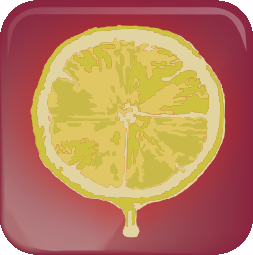
\includegraphics[width=2.5cm]{img/LOGO.png}
% \end{center}

%%%%%%%%%%%%%%%%%%%%%%%%%%%%%%%%%%
% 02_Installation
%%%%%%%%%%%%%%%%%%%%%%%%%%%%%%%%%%

\chapter{Installation}
\label{chap:Installation}

To obtain a local copy of SBMLsqueezer, you can download it in form of a 
\JAR from the project's website\footnote{Project website of SBMLsqueezer: \url{http://www.cogsys.cs.uni-tuebingen.de/software/SBMLsqueezer/}.}.

In the most common scenario, you might want to launch the program as a
stand-alone tool and access its \GUI. To do so,
start SBMLsqueezer with a simple double click on the icon of the downloaded
\JAR.
Provided that a \JVM is installed on your system 
(see \vref{sec:SoftwareRequirements}), you will see the main window of
SBMLsqueezer as soon as the splash screen has finished.

\section{Requirements}

SBMLsqueezer can be be used in multiple ways, depending on your preferences:
\begin{itemize}
  \item As a stand-alone tool
  \begin{itemize}
    \item via its \GUI (see \vref{chap:GUI})
    \item via its command-line interface (see \vref{chap:CMD})
  \end{itemize}
        In both cases, you can choose between \JSBML or \libSBML as your backend
        for \SBML (see \vref{sec:StandAlone}).
  \item As a plug-in for \CellDesigner (see \vref{sec:CellDesignerInstall})
  \item As a gadget for \Garuda (see \vref{sec:GarudaInstall})
  \item As an online program embedded in the Galaxy web service environment \citet{Goecks2010}
  \item As a \JavaWebStart application
  \item As a rate law core in an end-user application via its \API
\end{itemize}
Depending on how you like to use SBMLsqueezer, different requirements must be
fulfilled before launching the program for the first time.

Note that the extraction of kinetic equations from \SABIO requires an active Internet connection.
For this program features, the security settings of your \OS must also allow SBMLsqueezer to establish a connection to this online database.

When launching SBMLsqueezer, it will connect to the program homepage in order to check if a newer version of the program is available.
This feature can also only be used if an Internet connection is available and if your \OS allows SBMLsqueezer to establish such a connection.
Note that no further information is transmitted.
SBMLsqueezer only compares the version number of the local program with the version number of the latest release.
If you do not want to use this feature, you can switch it off.
See \vref{chap:CMD} for instructions how to do so.

\subsection{Hardware}

With at least 1\,GB main memory, you should be able to perform most tasks without any problem. For large models, you should have at least 2\,GB of main memory.
An active Internet connection is required for some program features, but not mandatory to run the program. %accessing the \SABIO database and to automatically obtain update information for SBMLsqueezer.

\subsection{Software}\label{sec:SoftwareRequirements}

SBMLsqueezer is entirely implemented in \Java and runs on any \OS, where a 
suitable \JVM, \JDK version~1.6 or newer, is installed.
For instructions how to obtain an up-to-date \JVM for your system, see, for 
example, the \Java SE download
page\footnote{\url{http://www.oracle.com/technetwork/java/javase/downloads/}\label{fn:jvmldl}}.

SBMLsqueezer has successfully been tested with
\begin{itemize}
  \item Microsoft \WindowsSeven Professional (64~bit),
  \item Microsoft \WindowsSeven Professional (SP1, 64~bit),
  \item \MacOSX (versions 10.8.2 through 10.10), and
  \item \UbuntuLinux (version 12.04, 64~bit).
\end{itemize}
See \vref{ch:faq} if you encounter any problems.

\section{Stand-alone application}
\label{sec:StandAlone}

Besides what is explained above, no further requirements are necessary if you
like to use SBMLsqueezer as a stand-alone application.
The program SBMLsqueezer does not have to be installed in order to be executed.
Just copy the \JAR of SBMLsqueezer to your preferred path on your hard-disk
to launch the application.
On \MacOSX, you may like to copy the \JAR into your
%\directory{Macintosh\textvisiblespace HD/Applications/}
\directory{Macintosh HD/Applications/}
folder.
On \Windows systems, the preferred position for the \JAR could be, for
instance,
%\directory{C:/Program\textvisiblespace Files/}
\directory{C:/Program Files/}.
For \Linux, we propose to copy the \JAR to the \directory{/opt/} folder.


\subsubsection{Using the \JSBML back-end}

No special actions are necessary if you like to use \JSBML, because this is the
default and \JSBML is already included in the \JAR that you have downloaded.

\subsubsection{Launching SBMLsqueezer with \libSBML as back-end}
\label{sec:UsingLibSBML}
Follow the installation instructions of the \Java binding for \libSBML for your
platform, which you can find at the website of
\libSBML\footnote{\url{http://sbml.org/Software/libSBML}}.
On some platforms, you may have to define an environment variable pointing
to the installation directory of \libSBML before being able to use its \Java
binding.
On the most \Unix and \Linux platforms, this variable is called
\LDLIBRARYPATH.
On \MacOSX, you should instead define the variable \DYLDLIBRARYPATH.
Follow the instructions at \libSBML's website\footnote{For information about how to execute a \libSBML-based \Java application, see the section about Java at \href{http://sbml.org/Software/libSBML/docs/cpp-api/libsbml-accessing.html}{\url{http://sbml.org/Software/libSBML/docs/cpp-api/libsbml-accessing.html}}} %#accessing-java
before launching SBMLsqueezer.
On Windows you should add the \libSBML directory to the \PATH environment in the Control Panel.
The following script can help you to to run SBMLsqueezer on your \Unix platform:
\begin{lstlisting}[language=bash, caption={Example Bash script that launches SBMLsqueezer with a \libSBML back-end}]
#!/bin/bash

VM_ARGS="-Xms32M -Xmx512M -Djava.library.path="
# The following lines depend on your system's configuration;
# so here is just an example:
VM_ARGS="${VM_ARGS}\
/usr/lib/jvm/java-6-sun/jre/lib/i386/client:\
/usr/lib/jvm/java-6-sun/jre/lib/i386:\
/usr/lib/jvm/java-6-sun/lib:\
/usr/local/lib"
#:[path to xerces]/xerces/lib
CLASS_PATH="/usr/local/share/java/libsbmlj.jar:\
[path to ]SBMLsqueezer_v2.0.1.jar"

# Set the environment variable; under Linux or most Unix systems this is
LD_LIBRARY_PATH="${LD_LIBRARY_PATH}:/usr/local/lib"
# On Mac OS you have to use the following code instead:
#DYLD_LIBRARY_PATH="${DYLD_LIBRARY_PATH}:/usr/local/lib"

# Start SBMLsqueezer using the command-line options:
MAIN_CLASS=org.sbml.squeezer.SBMLsqueezer 
java ${VM_ARGS} -cp ${CLASS_PATH} ${MAIN_CLASS} --try-loading-libsbml=true\
[further options]
\end{lstlisting}
In the example above the arguments for the \JVM define an initial heap space of
32~MB (\texttt{-Xms32M}) and a maximal heap size of 512~MB (\texttt{-Xmx512M}).
For more information about the program usage from the command line see \vref{sec:Program_usage}.


\section{Plug-in for \CellDesigner}
\label{sec:CellDesignerInstall}

If you like to use SBMLsqueezer as a plug-in for the popular graphical model
editor \CellDesigner \citep{Funahashi2003, Funahashi2006, Funahashi2007a, Funahashi2008}, you can do this by following four installation steps:
\begin{enumerate}
  \item Download and install \CellDesigner from the project's website\footnote{\url{http://celldesigner.org}}.
  \item Locate, where your copy of \CellDesigner is installed. 
  \item Open the \directory{plugin} folder in your installation of \CellDesigner and
        copy the file \file{SBMLsqueezer\_v2.0.1\_incl-libs.jar} into this folder.
  \item Open the \directory{lib} folder in your installation of \CellDesigner and
        replace the \JSBML \JAR that is redistributed by \CellDesigner with
        the \JAR \href{http://www.cogsys.cs.uni-tuebingen.de/software/SBMLsqueezer/downloads/jsbml-1.0-a1-with-dependencies.jar}{\url{jsbml-1.0-a1-with-dependencies.jar}}
        that you can download at \url{http://www.cogsys.cs.uni-tuebingen.de/software/SBMLsqueezer/downloads/}.
\end{enumerate}
Some more information about this installation procedure:
Depending on your \OS, \CellDesigner will be installed in different folders.
In \Windows it is usually
%\directory{C:/Program\textvisiblespace Files/CellDesigner4.4}
\directory{C:/Program Files/CellDesigner4.4}.
In \Linux you might find it in \directory{/opt/CellDesigner4.4}, and in \MacOSX \CellDesigner will be installed under
%\directory{Macintosh\textvisiblespace HD/Applications/CellDesigner4.4}
\directory{Macintosh HD/Applications/CellDesigner4.4}, where 4.4 is the version number with which SBMLsqueezer 2.0.1 has been tested.
Note that the version numbers 4.4 and 2.0.1 of \CellDesigner and SBMLsqueezer might change in the future, but the procedure will remain the same.

When replacing \CellDesigner's version of \JSBML with the one downloaded from the download site of the SBMLsqueezer project, 
make sure that the name of the new \JSBML file will be identical to the name of the \JSBML file distributed with \CellDesigner.
Otherwise, you will have to change some start script of \CellDesigner.
Even though this is not difficult and can be done on each \OS, we prefer to avoid that for the sake of simplicity.
Alternatively, you can also download \JSBML from the official \href{http://sourceforge.net/projects/jsbml/}{sourceforge} page.
However, you must make sure that the downloaded \JAR includes the package \directory{org.sbml.jsbml.celldesigner}.
Without this package, SBMLsqueezer cannot be launched in \CellDesigner.
Another possible solution is to checkout the development trunk of \JSBML and run the \ant script by yourself, thus building the latest version of \JSBML.
If you like to go this way, please read the documentation about \JSBML\footnote{\url{http://sbml.org/Software/JSBML/docs}} first.

It should be noted that SBMLsqueezer might produce different results when using it as a plug-in of \CellDesigner from the results of all other ways to use the program.
The reason is that \CellDesigner models can contain a rich tool-specific annotation, which can only be understood by SBMLsqueezer in the plug-in mode for this program.
In contrast, all other variants of SBMLsqueezer described herein depend on \SBO terms to indicate the roles of modifiers (e.g., enzymatic catalysts) when it is not used as a plug-in for \CellDesigner.
Again, the reason is that the \CellDesigner plug-in has different ways to receive this information.
Applying SBMLsqueezer to a model exported from \CellDesigner and opened in the stand-alone version might therefore yield different results compared to when directly running it as a plug-in from \CellDesigner.


\section{Integration into \Garuda}
\label{sec:GarudaInstall}

When downloading \Garuda, a functioning copy of SBMLsqueezer will be included.
Hence, no special installation steps are required. Just follow the instructions
of how to install \Garuda\footnote{\url{http://www.garuda-alliance.org/}} \citep{Ghosh2011}.

\section{Online program}
\label{sec:WebserviceInstallation}

In order to use SBMLsqueezer as an online program, it is necessary to install a recent web browser for your specific \OS, such as \href{http://www.mozilla.org}{Mozilla Firefox}, \href{https://www.google.com/intl/en/chrome/browser/}{Google Chrome}, \href{https://www.apple.com/safari/}{Apple Safari}, \href{http://windows.microsoft.com/en-us/internet-explorer/download-ie}{Microsoft Internet Explorer}, \href{http://www.opera.com/}{Opera}, or any other browser that you prefer and that is able to render up-to-date web sites.
See the documentation of Galaxy web services\footnote{\url{http://galaxyproject.org}} \citep{Goecks2010}, on which the online version of SBMLsqueezer is based, for precise software requirements.

When using the online version, no specific installation of SBMLsqueezer is necessary.
Note, however, that an active Internet connection is essential in order to use SBMLsqueezer as an online program.
Just use your regular web browser and go to \url{http://webservices.cs.uni-tuebingen.de} to use the program.
See \vref{sec:SBMLsqueezer_online_version} for further information.


%%%%%%%%%%%%%%%%%%%%%%%%%%%%%%%%%%
% 03_How to get started
%%%%%%%%%%%%%%%%%%%%%%%%%%%%%%%%%%

\chapter{How to get started}
\label{chap:GUI}

In this \namecref{chap:GUI} you will learn how the \GUI of the program
SBMLsqueezer is designed and intended to work, how you can launch, configure,
and use the program.
We will systematically go through all program features and explain what can be done and how.
Where possible, keystroke combinations will be introduced that can be used to simplify the work with the program.
All special scenarios of the diverse ways of using SBMLsqueezer (as a stand-alone tool, online program, plug-in in CellDesigner, \JavaWebStart application, as a gadget of \Garuda etc.) will be highlighted and discussed.

More experienced users might want to skip several parts of this \namecref{chap:GUI} and be more interested in the description of the command-line interface (see \vref{chap:CMD}) or examples for how to use the \API (see \vref{sec:API}) in custom applications.

\section{Starting the application}
\label{startingTheProgram}

\begin{wrapfigure}{O}{.9cm}
\vspace{\wrapfigspace}

\includegraphics[width=.8cm]{jar_icon}
\end{wrapfigure}
If you downloaded a \ZIP file, you need to unzip it before starting the application.
Launch SBMLsqueezer by double-clicking on the \Java icon, which might look like the
image next to this text, in a file browser of your \OS.
This will start the \GUI (see \vref{chap:GUI} for further details).

You can also start SBMLsqueezer from the command line.
Depending on your preference and your \OS, it might be helpful for
you to write a short shell or bash scripts for starting the application.
You might name this, for instance, \file{start.sh} for \Linux or \MacOSX, and
\file{start.bat} for \Windows. Within those scripts you could specify several
command-line options (see \vref{chap:CMD}) and hence customize the behavior of SBMLsqueezer.
How to do that is described in \vref{sec:Program_usage}.
If you are using \libSBML as your \SBML parsing engine, writing such a script is highly recommended.
You can find a sample script for this purpose in \vref{sec:UsingLibSBML}.

If you are using SBMLsqueezer as a plug-in for \CellDesigner, just open a model that you like to edit.
You can then launch all functions of SBMLsqueezer by clicking on one of the options within the menu
\menu{Plugin > SBMLsqueezer 2.0.1} in \CellDesigner.

\begin{wrapfigure}{O}{.9cm}
\vspace{\wrapfigspace}
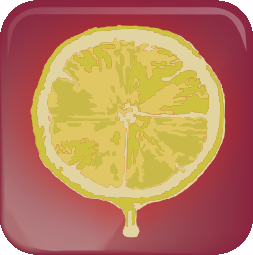
\includegraphics[width=.8cm]{img/LOGO}
\end{wrapfigure}
To start SBMLsqueezer in \Garuda, simply double-click on SBMLsqueezer's program icon (see the symbol that is printed next to this text).
Alternatively, you can also launch SBMLsqueezer there by sending an \SBML file to it from any other \Garuda gadget.
For more information about that, see the documentation of \Garuda.

When using SBMLsqueezer as an online program, just open a browser of your choice and go to \url{http://webservices.cs.uni-tuebingen.de} and select the tool SBMLsqueezer in the overview of tools.
You do not have to execute any further software besides your web browser.

\section{Adjusting the preferences}
\label{sec:GUIPrefs}

\begin{SCfigure}
\shadowimage[width=.5\textwidth]{prefs/Basic_configuration}
\caption[Basic configuration]{Basic configuration. All preferences %that you can manipulate
in this tab correspond to the command line options described in section~\ref{sec:Basic_configuration}.
You can specify if already existing rate laws should be replaced with newly generated ones, if a SABIO-RK search
should be performed etc. %and many more.
Taking small molecules and ions into account may lead to complex kinetic equations.
You can here give a list of KEGG %\citep{Kanehisa2000a}
identifiers for those species to be ignored when creating rate laws (see table~\ref{tab:MIRIAMignoreList}).
If values are missing in the model, this tab allows you to specify default values to be inserted. %Furthermore, 
You can decide how SBMLsqueezer should ensure unit consistency,
by either bringing all species to amount units, or to concentration units.
%Finally, 
For situations, in which the role of modifiers is unclear, you
can here select types of species to be considered enzymes.%
}\label{fig:BasicConf}
\end{SCfigure}
The program SBMLsqueezer offers a large number of options to configure how
kinetic equations are generated.
All options described in this section can also be applied using SBMLsqueezer's
command-line interface (see \vref{chap:CMD} for details).
This means that you can already upon launching the program define with which
options it should be initialized.
Your configuration can always be set back to the default options if desired.
SBMLsqueezer stores its configuration in the system's preferences of your \OS.
This means that when launching the program for the next time, you can directly
continue with your previous configuration.
Furthermore, there are no configuration files generated by SBMLsqueezer in
addition to those maintained by your \OS.
Hence, SBMLsqueezer integrates well into your working environment.

\begin{SCfigure}
\shadowimage[width=.5\textwidth]{prefs/Rate_law_selection}
\caption[Rate law selection]{Rate law selection.
It has been observed that irreversible rate laws are
often too restrictive and cannot capture the dynamics of complex reaction systems.
For this reason, SBMLsqueezer can create all kinetic equations in a reversible manner
and will then also update the property \emph{reversible} in affected reactions.
Depending on this setting, you will be able to select default types of irreversible
rate laws.
The other sections of this tab allow you to select which type of rate law should
be primarily selected when generating equations for an entire network in one single
step.
If you create equations for individual reactions only, as shown in \vref{fig:Rate_law_selection},
these settings do not have an effect.  
For more information about your choices in this tab, see also the description of
its corresponding command-line options in \vref{sec:Rate_law_selection}.}
\label{fig:Rate_law_selection}
\end{SCfigure}
\begin{wrapfigure}{O}{.9cm}
\vspace{\wrapfigspace}

\includegraphics[width=16px]{settings_64}
\end{wrapfigure}
We will now take a closer look at the options and describe what you can influence
and which choices the program offers to you.
In order to configure your preferences, you can click on the tool icon in the
tool-bar (see the icon next to this text), or select the corresponding entry in the menu bar.
Under \Windows and \Linux, you can access the preferences menu under
\menu{Edit > Preferences}, whereas
under \MacOSX, these can be found under \menu{SBMLsqueezer > Preferences\dots} or by using the keystroke
combination \keys{\cmd + {$,$}}.

\begin{SCfigure}
\shadowimage[width=.5\textwidth]{prefs/SABIO-RK_search_options}
\caption[\SABIO search options]{\SABIO search options.
The options in this tab correspond to the command-line options that are described
in \vref{sec:SABIO_search_options}.
You can specify general features of the reaction for which you want to look up
appropriate rate laws in \SABIO, such as the pathway, in which the reaction
occurs, the tissue, in which it was observed, even the cellular location.
Of course, you can also restrict your search to an organism of choice.}
\label{fig:SABIO-RK_search_options}
\end{SCfigure}
On the bottom panel of the preferences dialog you can see the four buttons
\keys{Cancel}, \keys{Defaults}, \keys{Apply}, and \keys{OK} as this is displayed in
\vrefrange{fig:BasicConf}{fig:LaTeX_Options}.
The \keys{Cancel} button has the same effect as a click on the close button on the
top of the window or hitting the \keys{\escwin} key: all of your changes will be
disregarded and the window will be closed.
The \keys{Defaults} button restores the standard settings of SBMLsqueezer.
With \keys{Apply} you can persistently save your current settings.
The \keys{OK} button is a combination of \keys{Apply} and close, i.e., it makes your
settings persistent and closes the window.
Hitting the \keys{\return} key has the same effect as clicking on the \keys{OK} button.
Note that the dialog is structured with multiple tabs. When clicking on
\keys{Defaults} the preferences in all tabs will be restored, even if those are not
active at the time when you hit that button.
\begin{SCfigure}
\shadowimage[width=.5\textwidth]{prefs/SABIO-RK_search_preferences}
\caption[\SABIO search preferences]{\SABIO search preferences.
All preferences in this tab can also be changed through the command line.
See \vref{sec:SABIO_search_preferences} for details.
Here you can define more fine-grained search search properties for looking up
kinetic equations in \SABIO, such as the minimal and maximal temperature and
pH value, under which the reaction proceeds, the currentness of the entry in
\SABIO, and several boolean switches that influence which type of database entry
can be considered.
These features are mainly important when extracting rate laws for all reactions
in the network in a bulk.
When you search for kinetics of individual reactions, you may want to also apply
more appropriate settings for just this reaction.}
\label{fig:SABIO-RK_search_preferences}
\end{SCfigure}
\begin{SCfigure}
\shadowimage[width=.5\textwidth]{prefs/LaTeX_Options}
\caption[\LaTeX{} options]{\LaTeX{} options.
All options in this tab are also available as command-line options
(see \vref{sec:LaTeX_Options}).
You can specify where your \LaTeX{} compiler is located in your \OS and what
to include into the model report.
This tab also gives you several style options that influence how the
the generated document will look like.
As a new feature, it now also supports the Layout extension for \SBML
\citep{Gauges2006}.
You can here decide if a figure of your network should be generated and
included into the report, given that layout information is provided in your file.
For more information about \SBMLLaTeX see the documentation of this project.}%
\label{fig:LaTeX_Options}
\end{SCfigure}


\section{Open a model}

\begin{wrapfigure}{O}{.9cm}
\vspace{\wrapfigspace}

\includegraphics[width=16px]{folder_64}
\end{wrapfigure}
The simplest way to open an \SBML file is to click on \menu{File > Open} in the
menu bar, or at the folder icon (see the icon next to this text) in the tool bar.
If you prefer keystroke combinations, you can use \keys{\cmd + O} on \MacOSX or
\keys{\ctrlwin + O} on \Windows and \Linux computers.
The \GUI can open multiple \SBML files in parallel.
SBMLsqueezer arranges these \SBML documents in tabs, whose order can be changed by dragging and dropping the tabs.
Furthermore, you can also open one ore multiple models in SBMLsqueezer via drag and drop, i.e., just select one or multiple \SBML files in an arbitrary file browser of your \OS and drag these into SBMLsqueezer's \GUI.

When starting SBMLsqueezer from the command line, you can directly pass a model
file to it, which will then be opened in the \GUI. To this
end, use the option \texttt{--sbml-in-file=<File>}, where \texttt{<File>} is the
absolute or relative path to the \SBML file you want to open (see
\vref{sec:IO_options}).
Note, however, that the command line option allows you to specify just one file
to open.
If you like to open further files, you need to do this in the \GUI.

In case that you use \libSBML as \SBML back-end, SBMLsqueezer will conduct a model validation upon opening the file.
The result of the validation will then be displayed in a dialog window.
This feature is not available when using \JSBML as \SBML back-end, because the \JSBML library does currently not implement an off-line validation for \SBML documents.

SBMLsqueezer remembers up to ten files you have already worked with.
Once you have opened one or more models, these are accessible in the menu bar,
where you can click on \menu{File > Recent files}.
This sub-menu will display the names of the files and their absolute path as tool-tip.
You can open one of these files by just clicking on its entry in the menu, or
you can apply one of the keystroke combinations \keys{\Altmac + 0} to \keys{\Altmac + 9}
on \MacOSX or \keys{\Altwin + 0} to \keys{\Altwin + 9} on \Linux and \Windows.
Here, the number keys are used to sort the previously opened models according to
when you last accessed the file.
The most recently opened file will always have number 0 and the model number 9
is the model that was opened a longer time ago.
Note that this order will change as soon as you open one model from this list
or any other model.

If you are working with \CellDesigner, open the model with this program's menu item or keystroke combination.
When launching the SBMLsqueezer as \CellDesigner plug-in, it will always use the currently selected model.
This means that, in case that you are working with multiple models in \CellDesigner, this model will be passed to SBMLsqueezer, whose tab is currently selected.

In \Garuda, SBMLsqueezer can receive files from other gadgets and will open these whenever this is requested.
SBMLsqueezer will automatically open accepted files.
There is hence nothing further to do.
If SBMLsqueezer is not running when a file is sent to it from another gadget, \Garuda will automatically launch the program and the file will be opened upon start.

\section{Equation generation one by one}
\label{sec:EquationsOneByOne}
\begin{SCfigure}
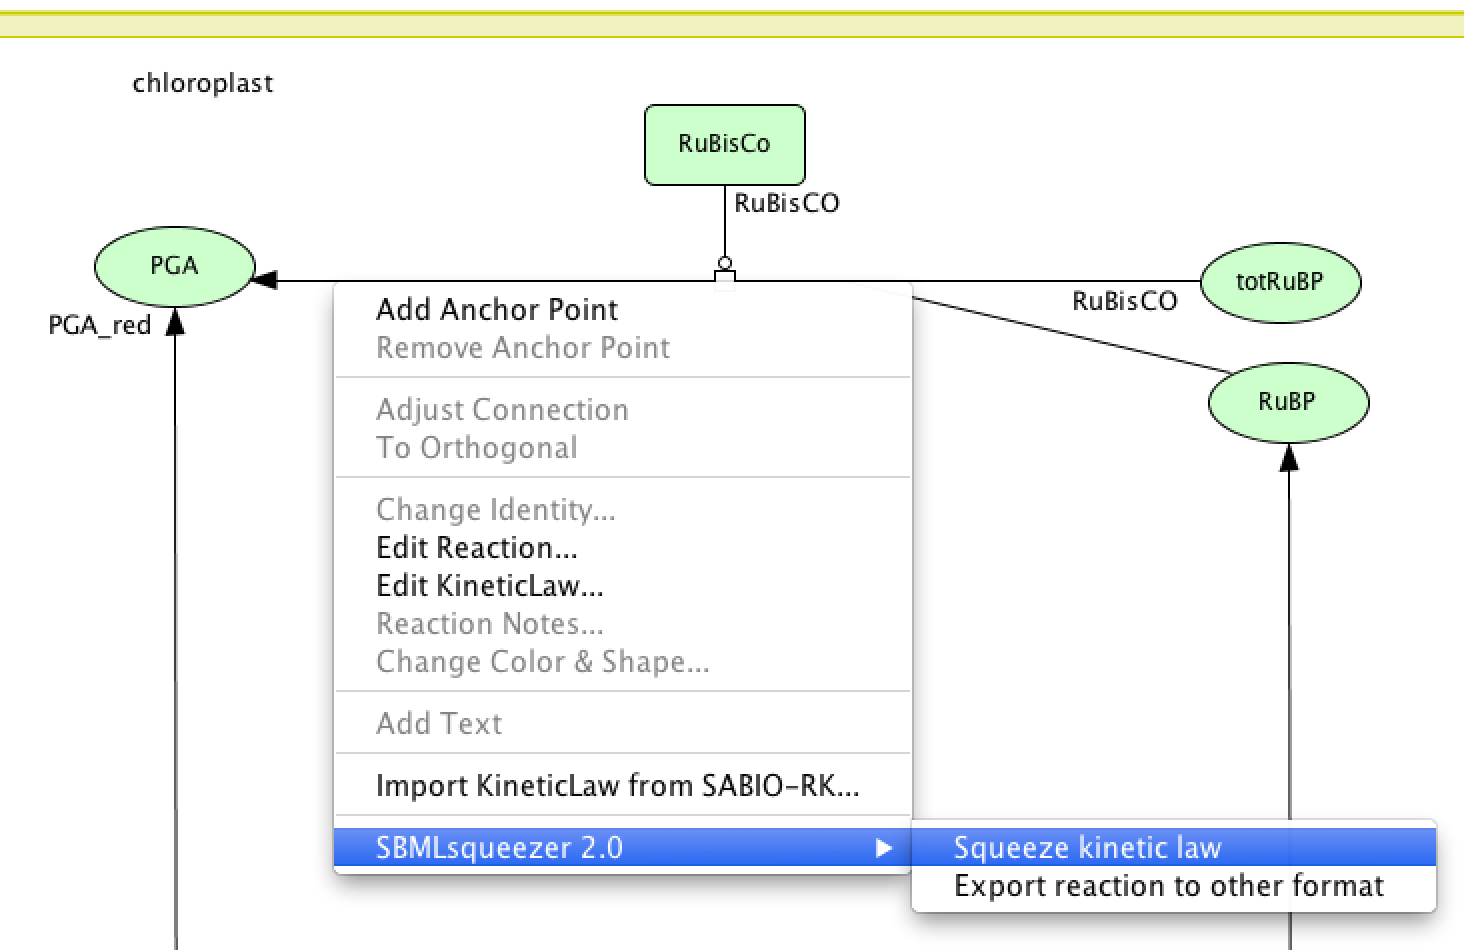
\includegraphics[width=.54\textwidth]{CellDesigner/reaction_context_menu.png}
\caption[Reaction context menu in \CellDesigner]{Reaction context menu in \CellDesigner.
After installing SBMLsqueezer as a plug-in, its functionality will be incorporated into \CellDesigner's reaction context menu.
If you right-click on an arbitrary reaction, it allows you to create a kinetic equation for this reaction (with the  dialog in \namecref{fig:RateLawDialog}~\ref{fig:RateLawDialog}), or to generate a \LaTeX{} model report that only involves the details relevant for the selected reaction.}
\label{fig:ReactionContextMenu}
\end{SCfigure}
\begin{figure}[b!]
\shadowimage[width=\textwidth]{Screenshot_2}
\caption[Generating a kinetic equation for a single reaction]{Generating a kinetic equation for a single reaction.
This dialog can be opened by right-clicking on an individual reaction in your active model and selecting \menu{Squeeze} in the pop-up menu.
%The equation preview displays how the rate law will look like, where zooming in and out can give you a better %overview.
The directionality of the reaction and the enzyme property can be altered.
%In most cases you can also decide if the reaction should be considered an enzyme reaction or not.
Both options possibly influence the selection of rate laws.
To abort this dialog, click on \keys{Cancel} or hit the \keys{\escwin} key.}
\label{fig:RateLawDialog}
\end{figure}

You can add a kinetic equation to individual reactions.
To this end, SBMLsqueezer provides a specialized context menu and dialog window, which enable you to select the type of rate law that seems appropriate for your purposes.
This dialog window is available whenever using SBMLsqueezer as a plug-in for \CellDesigner or in the stand-alone version (also in the \Garuda version).
In all cases, the same dialog window will appear, which offers you a selection of appropriate rate laws for the particular reaction and gives you the opportunity to choose between those, or to discard the dialog.
No change will be performed to your model when canceling the dialog (either by pushing \keys{\escwin} or by clicking on \keys{Cancel}).

We here use model \numero~390 from \BioModels \citep{Li2010a, Arnold2011} as an illustrative example.

In case that you are working with \CellDesigner \citep{Funahashi2003, Funahashi2006, Funahashi2007a, Funahashi2008}, right-click on the reaction of interest as this is displayed in \vref{fig:ReactionContextMenu} and select the menu item \menu{Squeeze kinetic law}.
When using SBMLsqueezer as a stand-alone program, you can generate kinetic equations for a selected reaction by right-clicking on the reaction of interest.
An example is given in \vref{fig:RateLawDialog}.
SBMLsqueezer analyzes the currently selected reaction according to various properties
and displays a selection of suitable rate laws, of which you can select
the most appropriate one.

The equation preview, where you can zoom in and out of the rendered formula, helps you to choose a rate law. If a corresponding \SBO entry can be found for a rate law, a tool-tip will be displayed with further information about this equation.
You can also decide if the reversibility of the reaction should be changed.
This would also alter the list of applicable kinetic equations.
The other options, if newly created
parameters should be locally attached to the kinetic law object or globally to
the model, influences the internal structure of the model, but not its behavior.
Just note, that there are some parameters, which cannot be stored locally because
they represent recurrent properties of some reactive species and are needed
across several rate laws (e.g., energy constants).

\section{Generate kinetic equations in a single step}

SBMLsqueezer can create rate laws for all reactions in one single step without the need of further human interaction or manual selection of rate laws for any reaction.
This option can %, for instance, 
be %very 
useful if you are working with a large model and want to create a first draft of a kinetic system, or if you are interested to apply the same type of approximative rate law to each reaction.
To see how to use this program feature, have a look at \vref{fig:KineticLawWizard}.

\begin{wrapfigure}{O}{.9cm}
\vspace{\wrapfigspace}

\includegraphics[width=16px]{SBMLsqueezerLogo_16}
\end{wrapfigure}
Just like in the case of the reaction context menu (\vref{sec:EquationsOneByOne}), the same kinetics wizard can be used in stand-alone mode and when working with the \CellDesigner plug-in version. % of SBMLsqueezer.
Various options allow you to customize how this is done.
The most important options decide if already existing rate laws should either be kept or overwritten, if all reactions can be modeled in a reversible manner, or as currently defined in the model.
In the \CellDesigner plug-in version, just click on \menu{Plugin > SBMLsqueezer 2.0.1 > Squeeze kinetic laws} to launch the kinetics wizard.
In the stand-alone version, you can either right-click on the model in the \SBML tree, the lemon icon in the tool bar (icon next to this text), or \menu{Edit > Squeeze} in the menu bar.

The usage of the kinetics wizard is identical, irrespective of how you launched it.
You can see how this wizard looks like in \vref{fig:KineticLawWizard}.
You can always discard all your changes by either clicking on the \keys{Cancel} button or by hitting the \keys{\escwin} key.
The \keys{Help} button opens a browser window that gives you more information about SBMLsqueezer.
If you click on \keys{Show options}, the preference dialog will be displayed, which is described in \vref{sec:GUIPrefs}.
In this way, SBMLsqueezer gives you the option to make sure that the selection of kinetic equations for all distinguished cases will be done as if you pick those individually.
\begin{SCfigure}
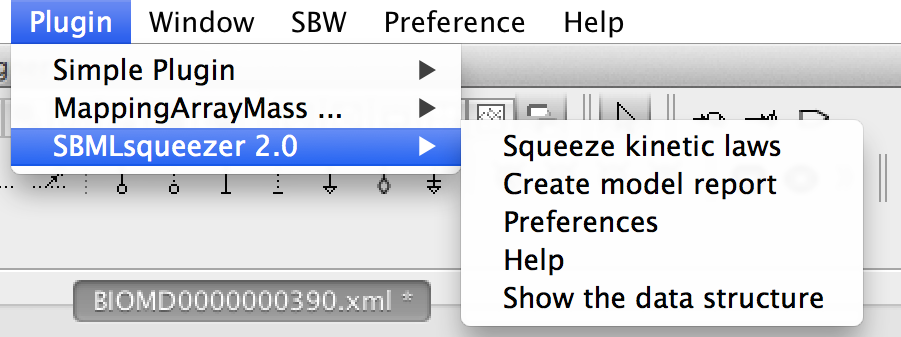
\includegraphics[width=.54\textwidth]{CellDesigner/plugin_menu}
\caption[Launching SBMLsqueezer in \CellDesigner]{Launching SBMLsqueezer in \CellDesigner.
The menu item \menu{Plugin > SBMLsqueezer 2.0.1} gives you access to nearly all functions of the program.
You can launch the kinetics wizard, adjust your preferences, export a \LaTeX{} report, open a help browser, or just look at how SBMLsqueezer internally represents \CellDesigner's data structure.}
\label{fig:PluginMenu}
\end{SCfigure}
\begin{figure}[b!]
\shadowimage[width=\textwidth]{Screenshot_4}
\caption[Generating kinetic equations in one single step with the kinetic law wizard]{Generating kinetic equations in one single step with the kinetic law wizard.
This screen-shot shows the Kinetic Law Wizard (here shown under \MacOSX).
When launched, this wizard allows you to generate kinetic equations for all reactions in the active model.
From this wizard, you can directly access and alter all program options, see the online help, and go back and forth between all steps through which the wizard will guide you.}
\label{fig:KineticLawWizard}
\end{figure}
\begin{figure}[t!]
\shadowimage[width=\textwidth]{wizard_results_table}
\caption[Results of the kinetics wizard displayed in a table]{Results of the kinetics wizard displayed in a table.
We again use model \numero~390 from \BioModels \citep{Li2010a, Arnold2011} as an example.
%In this example t
Two rows are highlighted in \colorbox{red}{red}.
The reason is that 
these reactions involve an unrealistically high number of reactant molecules, or are reversible with a high number of products, respectively.
These warnings indicate that the generated rate law might neglect several intermediate steps.
In this table, you can review all generated rate law.
Note that these will not be transferred to your original model before you hit the \keys{Finish} button.
You can alter each rate law by double- or right-clicking on an entry in the column ``Kinetic Law," or hit the \keys{Back} button and change your preferences for the rate law selection.
You can already generate a \LaTeX{} report about the changed model (hit the button \keys{Export changes}), which can help you to make your decision if you want to apply or discard your changes.}
\label{fig:wizard_results_table}
\end{figure}
\begin{SCfigure}[][b!]
\shadowimage[width=.64\textwidth]{Screenshot_8}
\caption[Changing selected rate laws in the kinetics wizard]{Changing selected rate laws in the kinetics wizard.
This dialog window appears when you double-click on an entry in the column ``Kinetic Law" of the kinetics wizard.
You can here select and apply an alternative rate equation.
If you want to change the criteria for the creation of equations, you need to go back to a previous step in the wizard.}
\label{fig:ChangingLawsInWizard}
\end{SCfigure}

When you hit the \keys{Next} button, kinetic equations will be created according to your settings and displayed in a summary table (see \vref{fig:wizard_results_table}).
You can change individual rate laws by double-clicking or right-clicking on a specific entry in this table.
A pop-up window will then appear asking you to choose an alternative rate law (see \vref{fig:ChangingLawsInWizard}).
When applying the change, the selection will be updated.
When you hit the button \keys{Finish}, the created rate equations, units, and parameter objects will be incorporated into your original model.

\section{Extraction of rate laws from \SABIO}

\begin{wrapfigure}{O}{.9cm}
\vspace{\wrapfigspace}

\includegraphics[width=16px]{SABIO}
\end{wrapfigure}
Instead of deriving kinetic equations \emph{de novo} for your model, you can also use SBMLsqueezer to automatically obtain experimentally determined equations from \SABIO.
To this end, SBMLsqueezer compares the reactions of interest to reaction signatures in this online database and allows you to select the most appropriate reactions or to restrict your search by using several parameters, such as pH, temperature etc.
Note that this feature does not apply for the \CellDesigner plug-in variant,
because \CellDesigner brings already with it its own \SABIO interface, which you can use directly in \CellDesigner.
Furthermore, this feature requires an active Internet connection and can therefore not be used in an off-line mode.

This section describes how to use the \GUI to extract information from \SABIO.
You can also do this on the command line, which allows for batch processing of multiple \SBML files as this has been done by \citet{Buechel2013}.
For more information about the command-line options for \SABIO see \vref{chap:CMD}.
You can directly use SBMLsqueezer's \API to benefit from this functionality. \Cref{sec:API} provides an elaborated description of how to use this feature.

\subsection{Rate laws from \SABIO for an entire network}
\label{sec:SABIOautomatic}

\begin{SCfigure}
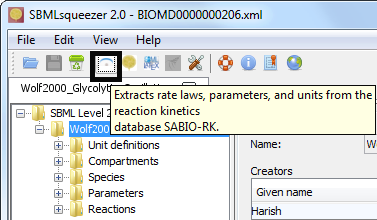
\includegraphics[width=.45\textwidth]{SABIO_automatic_1compact1}
\caption[Starting the \SABIO wizard]{Starting the \SABIO wizard.
After opening a model in SBMLsqueezer, the \SABIO button will become active in the tool-bar (see the black fringe).
A tool-tip will display more information about this button when moving the mouse over it.
You can click on this button to launch the \SABIO wizard.
Alternatively, you can also click on \menu{Edit > SABIO-RK}.}
\label{fig:startAutomatic}
\end{SCfigure}
\begin{SCfigure}
\shadowimage[width=.54\textwidth]{SABIO_automatic_2}
\caption[Selection of reactions in the \SABIO wizard]{Selection of reactions in the \SABIO wizard.
On the first window you can select which reactions you want to equip with kinetic equations from \SABIO. It is possible to directly select the reactions with some property (such as reactions not yet containing a kinetic law or fast reactions).
Furthermore, you can select the desired reactions by holding the \keys{\ctrlwin} key pressed while clicking on the desired reactions.
You can abort the wizard by either clicking on the \keys{Cancel} button or by hitting the \keys{\escwin} key.
When finished click on the button \keys{Next}.
\label{fig:selectReations}}
\end{SCfigure}
\begin{SCfigure}
\shadowimage[width=.54\textwidth]{SABIO_automatic_5}
\caption[Selection of search terms for \SABIO]{Selection of search terms for \SABIO.
On the next window you can add categories for search terms together with their values.
These terms are used to select only reactions and rate laws from \SABIO, whose annotation contains these terms.
An example is the organism, in which this reaction takes place.
You can choose ``organism" from the provided terms and type the desired name as value of the term in the text field.
By clicking on button \keys{Add} (black fringe), the term will be added to the table on the left-hand side of the dialog window.
See \vref{fig:removeSearchTerms} for an example how to remove a term again.}
\label{fig:searchTerms}
\end{SCfigure}
\begin{SCfigure}
\shadowimage[width=.54\textwidth]{SABIO_automatic_6}
\caption[Removal of search terms for \SABIO]{Removal of search terms for \SABIO.
You can remove a query field again by clicking on the check box button in the right-most column.
When you are done with selecting appropriate search terms, click on button \keys{Next} to see the results of your query. \Cref{fig:foundEquations} displays an example who this overview can look like.
The \keys{Back} button allows you to return to the selection of reactions as displayed in \vref{fig:selectReations}.
As before, you can abort the dialog by either hitting the key \keys{\escwin} or by clicking on the \keys{Cancel} button.
\label{fig:removeSearchTerms}}
\end{SCfigure}
\begin{figure}[b!]
\shadowimage[width=\textwidth]{SABIO_automatic_8compact}
\caption[Window with kinetic equations found for all reactions]{Window with found kinetic equations.
A reaction is highlighted in \colorbox{LimeGreen}{green} if a matching rate equation was found, \colorbox{Goldenrod}{yellow} if the found equations do not exactly fit to your model (there is no straightforward matching of all elements in the equation to elements in your model), and \colorbox{red}{red} if no matching rate equation was found.
If you are satisfied with the results, click \keys{Next}.}
\label{fig:foundEquations}
\end{figure}
\begin{figure}[t!]
\shadowimage[width=\textwidth]{SABIO_automatic_9compact}
\caption[Summary of necessary changes]{Summary of necessary changes.
The wizard summarizes all changes to the model that are required if you want to transfer the identified rate laws from \SABIO to your model.
This summary lists only changes related to reactions that have been highlighted in green in the previous step (\vref{fig:foundEquations}).
Upon clicking on \keys{Finish} a pop-up dialog will finally ask you to either confirm these changes to be made or to disregard all results.
If you confirm, the rate equations will be transferred to your model and all changes will be applied as stated in this summary.}
\label{fig:changes}
\end{figure}
\Crefrange{fig:startAutomatic}{fig:changes} show how you can add kinetic equations from \SABIO to several reactions at once.
As an example model we pick model \numero~206 from \BioModels \citep{Li2010a, Wolf2000}.
A wizard guides you through the selection of relevant reactions (\vref{fig:selectReations}) and provides several options to restrict the search in \SABIO (\vref{fig:searchTerms}), whose interface is similar to the database front end of \SABIO\footnote{\url{http://sabio.h-its.org}}.
To ensure that entries for the reactions of interest can be found in \SABIO, it is important to annotate these reactions with \acp{ID} from the \KEGG database \citep{Kanehisa2000a} using the \MIRIAM registry \citep{Juty2012}.
The \KEGG reaction \ac{ID} is then always included in the respective search in order to avoid adding kinetic laws referring to other reactions.
To further restrict your search, change the bounds of pH, temperature, etc. in the right panel (see \vref{fig:searchTerms}).

\subsection{\SABIO for a selected reaction}

\begin{figure}[t!]
\shadowimage[width=\textwidth]{SABIO_manual_1compact}
\caption[Starting the \SABIO application for a selected reaction]{Starting the \SABIO application for a selected reaction.
To find a reaction of interest, you can use the search function at the bottom of the \SBML tree.
Just click on the text field and type a part of the reaction's name or \ac{ID}.
The tree will be updated while you type and reduced to elements that contain the text you are typing.
Alternatively, you can just scroll to the entry of interest.
Once you have found a reaction of interest, right-click on it.
Then click on the \SABIO item in the pop-up menu and the \SABIO wizard will be started.
The reaction is shown again in the first window and you can just click on \keys{Next}.
This will bring you to the selection of search terms that is described in \vref{fig:searchTermsManual}.}
\label{fig:startManual}
\end{figure}
\begin{SCfigure}
\shadowimage[width=.54\textwidth]{SABIO_manual_3}
\caption[Selection of search terms]{Selection of search terms.
You can add search terms such as the organism by choosing from the provided terms and
typing in the value of the term. The search can be further restricted by changing the
bounds of pH, temperature, etc. in the right panel. 
You can remove a query field by clicking on the check-box button in the table on the left-hand side.
This dialog is just the same what has been described in \vrefrange{fig:searchTerms}{fig:removeSearchTerms} when adding kinetic laws to several reactions in a single step.
The example continues in \vref{fig:searchTermsQuery}.}
\label{fig:searchTermsManual}
\end{SCfigure}
\begin{SCfigure}
\shadowimage[width=.54\textwidth]{SABIO_manual_7}
\caption[Window with two search terms]{Window with two search terms.
Here a search for an organism and an enzyme name has been specified and will be
combined to a query when clicking on \keys{Next}.
You will then see the list of reactions as it is displayed in \vref{fig:foundEquationsManual}.}
\label{fig:searchTermsQuery}
\end{SCfigure}
As an alternative you can add kinetic equations from \SABIO to a selected individual reaction.
How to do this is shown in \vrefrange{fig:startManual}{fig:changesManual}.
We here use model \numero~206 from \BioModels \citep{Li2010a, Wolf2000} as an example network.
You should first select the reaction, for which you want to obtain a rate law from \SABIO (\vref{fig:startManual}).
All subsequent steps of the procedure are essentially the same as described before.
%when obtaining rate laws from \SABIO for all reactions in a single step.
The only difference is that the \SABIO wizard will be launched for one selected reaction of interest only instead of having all reactions in the model.
\begin{figure}[t!]
\shadowimage[width=\textwidth]{SABIO_manual_8}
\caption[Window with kinetic equations found for a single reaction]{Window with kinetic equations found for a single reaction.
The rate equations that match your search criteria are displayed here.
You can select a reaction and click on \keys{Next}, which will bring you to \vref{fig:matching}.
Alternatively, you can click on \keys{Back} and change your search criteria (see \vref{fig:searchTermsQuery}).
\label{fig:foundEquationsManual}}
\end{figure}
\begin{SCfigure}
\shadowimage[width=.54\textwidth]{SABIO_manual_9compact}
\caption[Window for matching elements in the equation to model elements]{Window for matching elements in the equation to model elements.
If kinetic laws are added to an entire network simultaneously, a straightforward matching of all elements (e.g., the species) contained in each rate equation to \SBML elements in your model will be necessary. 
In contrast to that, if you only add a rate law to one reaction at a time, the application presents you a suggestion for the matching and enables you to change it if desired. 
The necessary elements to import, such as function definitions contained in the rate equation to add, are also shown in this window.}
\label{fig:matching}
\end{SCfigure}
\begin{SCfigure}
\shadowimage[width=.54\textwidth]{SABIO_manual_10compact}
\caption[Summary of necessary changes]{Summary of necessary changes.
This overview summarizes how your model will be changed when adding the selected rate equation.
Now click on \keys{Finish} and afterwards a dialog pops up asking you to confirm the changes.
After this confirmation the rate equation will be transferred and these changes will be applied to your model.}
\label{fig:changesManual}
\end{SCfigure}


\section{Viewing and saving the results}

\begin{wrapfigure}{O}{.9cm}
\vspace{\wrapfigspace}

\includegraphics[width=16px]{save_64}
\end{wrapfigure}
When using the stand-alone version of SBMLsqueezer, you can see a tree representation of the \SBML document you are working with on the left-hand side of the \GUI.
\Cref{fig:Viewing_Results} displays how model \numero~390 from \BioModels \citep{Li2010a} looks like after SBMLsqueezer has modified one reaction's rate law.
The program recognizes if an \SBML document has been modified by one of its function.
You can see this because the title bar of the program will change, and the save actions in tool-bar and menu-bar will become active.
In \Windows and \Linux an asterisk will be added to the file name in the title bar.
In \MacOSX, the red ``close" button on the top-left most corner of the program will no longer display a cross, but a circle (you can see this in \vref{fig:Viewing_Results}).
You can save the modified file either by clicking on \menu{File > Save} or by clicking on the disk symbol in the tool-bar.
Alternatively, you can also use the keystroke combination \keys{\ctrlwin + S} (under \Windows and \Linux) or \keys{\cmd + S} (under \MacOSX).

You can always select \menu{File > Save as\ldots} in order to save the active \SBML document under a different file name.
The keystroke combination \keys{\shift + \ctrlwin + S} (\Windows and \Linux) \keys{\shift + \cmd + S} (\MacOSX) will also open a file chooser to save a copy of the active \SBML document.
In \MacOSX you have a further options to save the currently selected document elsewhere: you can drag the file symbol in the title bar into an arbitrary folder of a file browser.

Now, let us assume, you have used SBMLsqueezer to assign kinetic equations to the reactions in your model (either by extracting those from \SABIO or with the \emph{de novo} equation generator).
When expanding that tree and clicking on individual components, the program enables you to view the generated kinetic equations.
Just expand ``Reactions" and afterwards the desired reaction.
Then you can click on ``Kinetic law" and the rate equation is displayed on the right in detail.
A convenient search function at the bottom of the window helps you to quickly find reactions and other model components of interest.
\begin{figure}[t!]
\shadowimage[width=\textwidth]{Screenshot_7}
\caption[Viewing SBMLsqueezer's results]{Viewing SBMLsqueezer's results.
SBMLsqueezer provides a two-part view that displays the details of the model's structure.
On the left you can see the hierarchical \SBML data structure.
By clicking on selected elements within this tree, details about the element will be displayed on the right.
If you select a reaction or a kinetic law directly, the rate equation, parameters etc. will be displayed.
You can search for elements within the model by using the text field on the left-bottom corner.
This text field reacts to your input while typing and will immediately reduce the number of selectable items in the tree.
Exact hits will be highlighted in a bold font.}
\label{fig:Viewing_Results}
\end{figure}

When using SBMLsqueezer as a plug-in for \CellDesigner, you can either see the results by looking through the tables and overviews provided by \CellDesigner itself, or you can click on \menu{Plugin > SBMLsqueezer 2.0.1 > Show the data structure}. This will open a similar view as the stand-alone version provides.
SBMLsqueezer automatically synchronizes all of its changes with \CellDesigner.
This means that \CellDesigner will be notified about these changes and incorporate these into its in-memory model.
You can hence directly use its save functions or also save a copy of your model.

\section{Interaction with further \Garuda gadgets}
\begin{SCfigure}
\shadowimage[width=.45\textwidth]{Screenshot_9}
\caption[Selecting a \Garuda gadget]{Selecting a \Garuda gadget.
This dialog window shows you all available \Garuda gadgets that support the file type you are sending.
Upon hitting the \keys{OK} button, the model in the currently selected tab will be sent to the selected application.}
\label{fig:SelectGarudaGadget}
\end{SCfigure}

After having kinetic equations assigned to reactions of interest, it might be useful to pass the resulting \SBML document to further gadgets in \Garuda for subsequent analysis.
SBMLsqueezer is automatically connected to \Garuda core if it has been launched inside of \Garuda.
Otherwise, SBMLsqueezer will also connect to \Garuda if you launch your installation of \Garuda before starting SBMLsqueezer.
If SBMLsqueezer is already running when you launch \Garuda, no new connection will be established, you would need to restart SBMLsqueezer.

Now let us assume, your connection to \Garuda has been successfully established.
In this case, SBMLsqueezer can both, receive and send \SBML files from or to further gadgets.
SBMLsqueezer will notify you when it is connected to \Garuda by displaying a message in its status bar (at the bottom of the main window).
You do not have to do anything in SBMLsqueezer when you want to receive a file from another gadget.
The program will automatically be notified as soon as it receives the file and will directly open it in a new tab, so that you can work with the file as if you have just regularly opened it within the application.

It might, for instance, be an interesting idea to create a draft for a dynamic model directly based on information from the \KEGG database \citep{Kanehisa2000a} using \KEGGtranslator \citep{Wrzodek2011, Wrzodek2013} and to pass the model to SBMLsqueezer in order to assign kinetic equations. This model can then be forwarded to the application \SBMLsimulator \citep{Keller2013, Keller2014} that can be used to estimate the parameter values within the newly created kinetic laws, given that reference data are available.
A similar approach has been suggested for the generation of draft genome-scale metabolic models \citep{Buechel2013}.

\begin{wrapfigure}{O}{.9cm}
\vspace{\wrapfigspace}

\includegraphics[width=16px]{ICON_GARUDA_48}
\end{wrapfigure}
As soon as at least one \SBML file has been opened, SBMLsqueezer will activate the \Garuda icon in the tool-bar (which you can see next to this text) as well as the menu item \menu{File > Send current file to Garuda}.
By clicking on that icon or selecting this entry in the menu bar, you can send the active file, i.e., the file that belongs to the currently selected tab in SBMLsqueezer, to another gadget.
To this end, SBMLsqueezer will display the dialog window that is shown in \vref{fig:SelectGarudaGadget}.
If the model in the selected tab has been modified and not yet saved, SBMLsqueezer will create a temporary file in your \OS's directory for temporary files and send this file to the selected gadget.

\section{Using SBMLsqueezer as an online program}
\label{sec:SBMLsqueezer_online_version}

SBMLsqueezer can also be used via the Galaxy web service facility \citep{Goecks2010} of the University of Tuebingen\footnote{\url{http://webservices.cs.uni-tuebingen.de}\label{fn:Webservices}}.
Since the user interface of this variant greatly differs from all other use-case scenarios, we here give a description of options and functions of the web interface.

In order to use the online version of SBMLsqueezer, open a browser of your choice.
Go to the main portal of all web services provided by the Universtiy of Tuebingen\footref{fn:Webservices}
and scroll down until you find the tool SBMLsqueezer and click on the the program's logo, or you can click on the link in the list of tools on the left.
Alternatively, you can directly go to the service SBMLsqueezer\footnote{\url{http://webservices.cs.uni-tuebingen.de/tool_runner?tool_id=sbmlupload2}}.
\Cref{fig:WebserviceLaunch} displays the web interface of the \Galaxy framework \citep{Goecks2010}.
\begin{figure}
\shadowimage[width=\textwidth]{Webservice/SBMLsqueezerWebservice1}
\caption[Starting the online version of SBMLsqueezer]{Starting the online version of SBMLsqueezer.
This figure displays the Galaxy framework in the browser Firefox (version 29.0.1) under \MacOSX (version 10.9.3).
You can start working with SBMLsqueezer by either clicking on the program's icon or the link ``Upload SBML file".}
\label{fig:WebserviceLaunch}
\end{figure}

The first step is now to upload your \SBML file of interest to the online program.
To this end, you can either click on the link ``Upload SBML file" on the left-hand side of the browser window, or click on the icon of SBMLsquezeer.
In both cases you should see a browse button that allows you to select an \XML or \SBML file from your local file system.
After selecting the file, hit the button ``Execute" in order to actually upload the file to the Galaxy service.
Galaxy informs you about the progress of the upload in the ``History" column at the right-hand side of the browser window.
You can upload further files if you like, but at least one file is required in order to run SBMLsqueezer.
Please note that uploaded models and files will be deleted after the job has been executed and are not accessible to any third-parties, i.e., data security is guaranteed.

Second, click on the link ``Generate kinetic rate equations" on the left-hand side of the browser window.
You should see a view similar to what is displayed in \vref{fig:WebserviceConfiguration}.
Scroll down to see all available options.
At the bottom of this page, there is also a descriptive text explaining how to proceed.
Each option has descriptive text as well.
The online version presents all options of the program just as the stand-alone version.
You can therefore go back in this tutorial and look-up the meaning of individual options either in \vref{sec:GUIPrefs} about the \GUI of the stand-alone version or in \vref{chap:CMD} where the command-line options are described.
When you scroll down, you can see that this online program also offers you to obtain rate laws from \SABIO.
Just one option group is missing, namely \SBMLLaTeX.
The reason is because the Galaxy framework of the University of Tuebingen provides \SBMLLaTeX as a separate online program \citep{Draeger2009b}.

When you are happy with the settings, scroll down until you see the ``Execute" button.
When you hit this button, SBMLsqueezer will create kinetic equations for your model according to your preferences.
To this end, a new job will be scheduled that will be displayed in your history.
\begin{figure}
\shadowimage[width=\textwidth]{Webservice/SBMLsqueezerWebservice2}
\caption[Adjusting preferences in the online version]{Adjusting preferences in the online version.
In this example, three models have been uploaded to the Galaxy service and are shown in the history column in the right-hand side of the browser window.
You can now choose for which file SBMLsqueezer should generate kinetic equations by altering the selected entry in the combo box at the top of the center column.
In the center column, this view offers you all options of the stand-alone version of SBMLsqueezer.}
\label{fig:WebserviceConfiguration}
\end{figure}

When the job is done, you can obtain the results by first clicking on the link ``Generated kinetics for [file name]," which will appear in the history column.
You can then click on the disk icon below in order to download the \SBML file that contains your results.
If you click on the eye icon, the central column will display a rendered version of your \SBML file, which is the view at all \XHTML notes within your file.
\begin{figure}
\shadowimage[width=\textwidth]{Webservice/SBMLsqueezerWebservice3}
\caption[Obtaining the results from the online version]{Obtaining the results from the online version.
The history column contains an overview of all files for which kinetic equations have been generated.
You can view the details of each file by clicking on the eye icon, or download the file by first clicking on the link in the headline of the respective entry (``Generated kinetics for\ldots") and then clicking on the disk icon.}
\label{fig:WebserviceResult}
\end{figure}

\chapter{Advanced program features}
\label{chap:AdvancedFeatures}

This \namecref{chap:AdvancedFeatures} discusses how more experienced users can benefit from SBMLsqueezer's capabilities.
%This includes a large variety of command-line options and also the elaborated \API.
In the first two \namecref{sec:API}s we will have a look behind the scenes and explain how you can directly access and use the \API of SBMLsqueezer in a programming environment.
In the next \namecref{chap:CMD} we will list and explain all possible command-line options.
All program features that have been described in the previous \namecref{chap:GUI} can also be addressed through the command-line and programming interface, making SBMLsqueezer a versatile tool that can be used in diverse, customized applications.

\section{Using SBMLsqueezer as an equation generator library}
\label{sec:API}

We will now discuss how to use the \API of SBMLsqueezer directly in order to generate kinetic equations as part of more complex operations.
This function could already be used in version 1.3 of SBMLsqueezer (see \vref{lst:1.3APIUsage}).
Since then, the \API has been greatly modified and improved.
We will now discuss important aspects of the new \API of SBMLsqueezer and give examples of particularly important use-case scenarios.

\subsection{Assignment of kinetic equations to all reactions in an \SBML file}

\Cref{lst:SBMLsqueezer2API1} gives you an example for a simple application that takes the paths to two \SBML files as input and proceeds as follows:
\begin{enumerate}
  \item It changes the preferences of the program by defining several options.
  \item It creates an instance of \texttt{SBMLsqueezer} with type parameter \texttt{org.sbml.jsbml.Model}, i.e., it will use \JSBML as its parsing library.
  \item By calling the \texttt{squeeze} method, it will then use \JSBML to read the first file into an \texttt{SBMLDocument} data structure and generate kinetic equations for all reactions within the document according to the current preferences.
  \item The result will be written into the second file, i.e., the original file will remain unchanged unless the two arguments point both to the identical file.
\end{enumerate}
The paths in this example can also point to a directory instead of a particular file.
If this is the case, \texttt{SBMLsqueezer} will recursively traverse all acceptable \SBML files in the given input folder and create a corresponding file with newly created or obtained kinetic equations in the output folder.
\lstinputlisting[caption={Generating rate laws for all reactions in a model via the \acs{API} of SBMLsqueezer 2}, label={lst:SBMLsqueezer2API1}, firstline={45}, lastline={77}]{../../../examples/src/org/sbml/squeezer/test/SqueezeFile.java}

\subsection{Adjusting configuration and user preferences}

While the previous version of SBMLsqueezer stored its preferences in configuration files within the user's home directory, SBMLsqueezer now makes use of the preferences of your \OS.
The keywords for the individual options have been slightly changed, but are still very similar.
In general, the names of the command-line options (see \vref{chap:CMD}) are very similar to the names of the options that you can use when hacking SBMLsqueezer's \API.
Furthermore, the grouping of the preferences is identical to the grouping of options you have in the tabs of the preferences dialog (see \vrefrange{fig:BasicConf}{fig:LaTeX_Options}) and also the groups of command-line options.
You can therefore read through the command-line options in order to get a description of potential options to be used in the \API.
The \Java \API documentation, which you can find online on the project's homepage\footnote{\url{http://www.cogsys.cs.uni-tuebingen.de/software/SBMLsqueezer/doc/api/SBMLsqueezer2.0.1/}}, will also be helpful to gain an understanding of available options.

The options of SBMLsqueezer are each gathered in specialized interfaces, which all extend the interface \texttt{KeyProvider}.
Each option is a constant field variable.
If you are using an \IDE, such as \Eclipse, an auto-complete function will directly show you which options are provided within a particular sub-class of \texttt{KeyProvider}.
Such an \IDE will also display the Java documentation to you.
You can load the preferences by calling
\begin{lstlisting}[language=Java, numbers=none, caption={Loading preferences in SBMLsqueezer 2}]
SBPreferences prefs = SBPreferences.getPreferencesFor(MyOptionsClass.class);
\end{lstlisting}
Here, \texttt{MyOptionsClass} acts as a placeholder for your actual instance of \texttt{KeyProvider} for which you want to load preferences.
SBMLsqueezer gathers its specific options in the following interfaces:
\renewcommand{\descriptionlabel}[1]{\textcolor{blue}{\texttt{#1}}}
\begin{description}
  \item[org.sbml.squeezer.OptionsGeneral] See the command-line options described in \vref{sec:Basic_configuration}.
  \item[org.sbml.squeezer.io.IOOptions] These options are described in \vref{sec:IO_options}.
  \item[org.sbml.squeezer.kinetics.OptionsRateLaws] Corresponds to the command-line arguments in \vref{sec:Rate_law_selection}.
  \item[org.sbml.squeezer.sabiork.SABIORKOptions] See the description in \vref{sec:SABIO_search_options}.
  \item[org.sbml.squeezer.sabiork.SABIORKPreferences] See \vref{sec:SABIO_search_preferences}.
\end{description}
Each option has a specific data type associated with it.
You can hence use a call of the \texttt{put} method on your instance of \texttt{SBPreferences} to alter the value
for an option.
Thereby, the option is used as the key in the preferences object.
In the same way, you can also obtain the current value for an option.
Just read the documentation about preferences of the standard \Java distribution\footnote{\url{http://docs.oracle.com/javase/6/docs/api/java/util/prefs/Preferences.html}}.
The only difference is that SBMLsqueezer uses an extended version of the regular preferences implementation, which allows you to directly store and retrieve more complex data structures besides \texttt{String}s, such as \texttt{File} or \texttt{Class} objects.
In particular, when selecting a specific kind of rate law for a certain type of reaction, SBMLsqueezer expects the class object of that \texttt{KineticLaw}.
Note that this is in contrast to version~1.3, which expected the name of the class.

\subsection{Using SBMLsqueezer with a \libSBML back-end}


Let us now discuss how you can use SBMLsqueezer's \API with a \libSBML back-end instead of pure \JSBML.
To this end, you only have to change the way how you initialize your instance of \texttt{SBMLsqueezer}:
\begin{lstlisting}[language=Java, numbers=none, caption={Initializing SBMLsqueezer 2 with a \libSBML back-end}]
SBMLsqueezer<org.sbml.libsbml.Model> squeezer = new SBMLsqueezer<org.sbml.libsbml.Model>(
  new org.sbml.jsbml.xml.libsbml.LibSBMLReader(),
  new org.sbml.jsbml.xml.libsbml.LibSBMLWriter());
\end{lstlisting}
Everything else of \vref{lst:SBMLsqueezer2API1} can be left unchanged.
Here, we are initializing \texttt{SBMLsqueezer} based on a \libSBML \texttt{Model} data structure.
It is important to use the correct reader and writer from the package \texttt{org.sbml.jsbml.xml.libsbml}, and not to confuse these with the \texttt{LibSBMLReader} and \texttt{LibSBMLWriter} from the \texttt{org.sbml.jsbml.celldesigner.libsbml} package in \JSBML.
Otherwise, your application will not function, because the classes in this package are very basic implementations needed for the interface between \JSBML and \CellDesigner.

Please note that SBMLsqueezer can internally only work with the \JSBML data structure.
The \libSBML back-end is used to parse and write \SBML files and also allows for off-line model validation.
However, SBMLsqueezer will convert \libSBML's data structure to \JSBML and synchronize its changes to the original data structure.
When run-time is crucial for your application, this procedure should hence be avoided.

\subsection{Assignment of specific rate laws to selected reactions}

Instead of reading and writing entire files or recursively walking through a directory structure, it can also be desirable to perform more customized calls to create rate laws for individual reactions only.
To this end, a deeper understanding about the functioning of SBMLsqueezer is required.
There are a few particularly important classes for the \emph{de novo} creation of kinetic equations, which are all located in the package \texttt{org.sbml.squeezer}:
\begin{description}
  \item[KineticLawGenerator] This class contains the actual algorithms to build a rate law and to synchronize changes between models.
  \item[ParameterFactory]
    Here all (local) parameters are generated.
    The implementation follows the factory pattern, but it requires an instance of the model for which the parameters are created because of numerous dependencies between objects and \acp{ID}.
    It uses the unit factory (see below) to derive the units of new parameters.
    This class also annotates all newly created parameter objects with \SBO terms.
  \item[SubmodelController]
    SBMLsqueezer never modifies the original model data structure.
    Internally, this controller creates a minimal copy of the model, only comprising those reactions with dependent model components (required species, compartments, parameters, units etc.) that are needed to work with the currently selected set of reactions.
    In the \GUI, the user can typically select one or all reactions of a model.
    This class is more powerful, as it could potentially generate a sub-model for an arbitrary set of reactions with all required other components of the model.
    It hence generates a restricted clone of the model.
  \item[ReactionType]
    This class determines the base type of a given reaction and contains the algorithms that select appropriate rate laws or the most suitable rate law.
    It also removes substances from the reaction if these belong to the group of substances from the ignore list (see  \vref{tab:MIRIAMignoreList}).
  \item[UnitFactory]
    This factory class generates unit definition objects and \acp{ID} for unit definitions, which are to be assigned to parameters and numbers in kinetic expressions.
\end{description}
\renewcommand{\descriptionlabel}[1]{\textcolor{black}{\textbf{#1}}}
With these classes at hand, new kinetic equations can be created for arbitrary reactions.
The example in \vref{lst:SBMLsqueezer2API1} demonstrates how a convenience rate law \citep{Liebermeister2006} can be assigned to a selected reaction in an \SBML file.
This type of rate equation can be applied to reversible as well as to irreversible enzyme-catalyzed reactions and has been found to be particularly useful when no specific information about reaction mechanisms is known \citep{Draeger2007b, Draeger2009a, Draeger2011a}.
\lstinputlisting[caption={Assignment of a kinetic law to a reaction via the \acs{API} of SBMLsqueezer~2}, label={lst:SBMLsqueezer2API2}, firstline={47}, lastline={76}]{../../../examples/src/org/sbml/squeezer/test/SqueezeReaction.java}

\section{Querying \SABIO and merging the results into a local \acs{SBML} document}

The command-line mode for the interface to \SABIO is implemented in the class \texttt{ConsoleWizard}.
This class is located in the package \texttt{org.sbml.squeezer.sabiork.wizard.console}.
The following example shows how to query for rate equations in \SABIO by using SBMLsqueezer's \API.
The search can either comprise all reactions or just the reactions in a model.
All search terms that can be applied to the model are listed at the beginning of the source-code example.
The \KEGG \citep{Kanehisa2000a} \ac{ID} of a reaction is automatically added to the search terms (compare \vref{sec:SABIOautomatic}).
A found kinetic law is added to a reaction if all contained elements can be matched to \SBML elements in the model.
\lstinputlisting[caption={\SABIO query for the reactions of a model}, label={lst:SBMLsqueezer2API3}, firstline={100}, lastline={141}]{../../../examples/src/org/sbml/squeezer/test/SABIORKApplication.java}

You can also launch the \GUI of the \SABIO wizard by using SBMLsqueezer's \API.
The following source-code example demonstrates how to do so.
\lstinputlisting[caption={Calling the \SABIO wizard}, label={lst:SBMLsqueezer2API4}, firstline={52}, lastline={98}]{../../../examples/src/org/sbml/squeezer/test/SABIORKApplication.java}


%\chapter{Example use cases}
%
%\section{\emph{De-novo} creation of kinetic equations}
%\subsection{For an entire network}
%Starting from the screen in \vref{fig:KineticLawWizard} you have to click on \keys{Next}. On the next screen you see a table with the reactions and the suggested type of rate equation for each reaction (\vref{fig:suggestedEquations}). You can change a suggested rate law, if you are not satisfied with it (see \vref{fig:changeEquation}).
%
%\begin{figure}[htbp]
%\shadowimage[width=\textwidth]{Screenshot_5}
%\caption[Table with suggested rate equation types]{Table with suggested rate equation types.
%This table is displayed, when you start from the screen in \vref{fig:KineticLawWizard} and click on \keys{Next}. The table shows which type of rate equation SBMLsqueezer suggests to generate for each reaction as well as a preview of the respective formula. You can add the rate laws to the model by clicking on \keys{Finish}.}
%\label{fig:suggestedEquations}
%\end{figure}
%
%\begin{SCfigure}
%\shadowimage[width=.54\textwidth]{Screenshot_6}
%\caption[Choosing an alternative rate law]{Choosing an alternative rate law.
%If you are not satisfied with a rate law type suggested by SBMLsqueezer, you can click on the respective row in the table in \vref{fig:suggestedEquations}. Then this window is displayed which lets you choose another type of rate law.}
%\label{fig:changeEquation}
%\end{SCfigure}
%
%\subsection{For selected reactions}
%You can generate a rate law for a specific reaction by right-clicking on it. Then a window appears, which lets you choose the type of rate law (see \vref{fig:RateLawDialog} for details).


\section{Command-line arguments}
\label{chap:CMD}
\renewcommand{\descriptionlabel}[1]{\textcolor{blue}{\texttt{#1}}}

All functions of the program SBMLsqueezer are also available as command-line
arguments. SBMLsqueezer is therefore fully functional even if you do not use
its \GUI.
This can be useful if you like to generate kinetic equations, units, and
parameter objects for a large number of \SBML files in a loop or in a more
complex schedule.
To benefit from this functionality, just open a command line window on your
\OS, e.g., execute the \file{cmd.exe} in \Windows or open a terminal window
in \Unix (incl. \Linux and \MacOSX).

It should also be noted that the command line options impact the \GUI.
It is hence possible to use command-line options in order to launch
SBMLsqueezer with a pre-defined configuration.
However, you should note that if you pass a command-line argument to SBMLsqueezer, it might assume that you intend to use the program in the pure command-line mode and hence will not launch the \GUI.
In this case, you will need to also pass the command-line option  \texttt{--gui=true} or just \texttt{--gui} to the program.

\subsection{Program usage}
\label{sec:Program_usage}

You can start the application on all {\OS}s by typing
\begin{lstlisting}[language=bash, numbers=none, caption={Launching SBMLsqueezer from the command-line}]
java -jar SBMLsqueezer.jar [options]
\end{lstlisting}
on your command prompt. Please note that you might have to change
\file{SBMLsqueezer.jar} for the real name of the \JAR, e.g.,
\file{SBMLsqueezer\_v2.0.1\_incl-libs.jar}.
For future versions of SBMLsqueezer the name of the
\JAR could also change, because it usually includes the version number.

In most cases, SBMLsqueezer needs more than 128\,MB memory, so it might be convenient to create a
shortcut and start the application with as much memory as available. If you
have 2\,GB RAM, for example, you might want to start the application with the
following command:
\begin{lstlisting}[language=bash, numbers=none, caption={Launching SBMLsqueezer from the command-line with increased heap size}]
java -Xms128m -Xmx1400M -jar SBMLsqueezer.jar [options]
\end{lstlisting}
How much memory you actually need strongly depends on the size of your input datasets.
Under \Windows you might want to type \texttt{javaw} instead of \texttt{java} in order to be able to close
the command-line window while the program is running.
This feature is particularly useful when writing a batch script to launch SBMLsqueezer with your favorite command-line arguments.

Use the following program parameters to lists all available options of
SBMLsqueezer: \texttt{--help} or \texttt{-?}.
The subsequent sections describe all available options of SBMLsqueezer
version~2.0.1.

SBMLsqueezer's entire user interface (the \GUI as well as the command line) is equipped
with with language packs for \German and \English, and partially for \Chinese (Mandarin).
By default the program checks your system's configuration and loads the language pack of
your operating system.
The fallback language is \English.
You can also purposely choose the language of the user interface by passing the language parameter as an
argument to the \JVM.
To this end use the following launch command
\begin{lstlisting}[language=bash, numbers=none, caption={Launching SBMLsqueezer with an alternative language pack}]
java -Xms128m -Xmx1400M -Duser.language=en -jar SBMLsqueezer.jar [options]
\end{lstlisting}
if you want to launch the program with an \English user interface.
For \German use \texttt{de}, and \texttt{zh} for \Chinese.

\subsection{Input/output options}
\label{sec:IO_options}
\begin{description}
\item[--sbml-in-file{[} |={]}<File>]
  Specifies the \SBML input file.
  Default value: none

\item[--sbml-out-file{[} |={]}<File>]
  Specifies the file where SBMLsqueezer writes its \SBML output.
  Default value: none

\item[--try-loading-libsbml]
  If selected, the application will try to load the library \libSBML
  for reading and writing \SBML files, otherwise everything will
  be done with \JSBML only, i.e., pure \Java and therefore platform independent.
  Default value: \texttt{false}
\end{description}

\subsection{Basic configuration}
\label{sec:Basic_configuration}
With the options introduced in this section, you can specify which assumptions
SBMLsqueezer should make when values or information are missing, i.e., if the 
model is lacking more information than just kinetic equations. You can also
specify how to interpret the model and when error messages should be displayed.

\subsubsection{General Options}
The behavior of SBMLsqueezer can be specified by the following options, for
instance, to decide if error messages should be displayed under
certain circumstances.
\begin{description}
\item[--overwrite-existing-rate-laws{[} |={]}<Boolean>]
  If this flag is set to \texttt{true}, a new rate law will be created for
  each reaction irrespective of whether there is already a rate
  law assigned to this reaction or not. If \texttt{false}, new
  rate laws are only generated if missing in the \SBML file. Note
  that if this option is checked, already existing kinetic laws
  will be overwritten.
  Default value: \texttt{true}

\item[--set-boundary-condition-for-genes{[} |={]}<Boolean>]
  If \texttt{true}, the boundary condition of all species that
  represent gene-coding elements, such as genes or gene coding
  regions, will be set to \texttt{true}.
  Default value: \texttt{true}

\item[--all-reactions-as-enzyme-catalyzed{[} |={]}<Boolean>]
  If \texttt{true}, all reactions within the network are considered to be
  enzyme-catalyzed reactions. If \texttt{false}, an explicit
  enzymatic catalyst must be assigned to a reaction to obtain
  this status.
  Default value: \texttt{true}

\item[--remove-unnecessary-parameters-and-units{[} |={]}<Boolean>]
  If \texttt{true}, parameters and units that are never referenced
  by any element of the model are automatically deleted after
  creating kinetic equations.
  Default value: \texttt{true}

\item[--new-parameters-global]
  If \texttt{true}, all parameters are stored globally for the
  whole model. Otherwise the majority of parameters is stored
  locally for the respective kinetic equation they belong to.
  Note that some parameters represent global properties of the
  entire model and should therefore be always stored in the global
  list of parameters. In this way, these parameters are valid within
  the entire model.
  Default value: \texttt{false}

\item[--warnings-for-too-many-reactants{[} |={]}<Boolean>]
  If \texttt{true}, warnings will be displayed for reactions with
  an unrealistic number of reactants. The maximal number of reactants
  that are believed to be still realistic can be defined if this
  option is selected.
  Default value: \texttt{true}

\item[--show-sbml-warnings{[} |={]}<Boolean>]
  If \texttt{true}, \SBML warnings are displayed. These warnings are
  mainly the result of a syntactical model check and do not give much
  information about the semantic correctness of your model.
  Since the \SBML library performs this check, SBMLsqueezer cannot influence the
  content of the syntax check. Note that this option only works properly if you
  use \libSBML as your \SBML back-end, because \JSBML does not provide a full
  validity check for \SBML models.
  Default value: \texttt{true}

\item[--read-from-sabio-rk{[} |={]}<Boolean>]
  This option lets the user choose whether to search for experimentally
  obtained rate laws in the reaction kinetics database \SABIO. Note that
  performing this search requires an active Internet connection.
  Default value: \texttt{true}
\end{description}

\subsubsection{Default values}

The options in this group allow you to specify several default values to be
applied for components of the model.
This is done in addition to the actual rate law generation, such as the default
compartment size etc., and to define model wide settings to be taken into
account when creating rate equations.
\begin{description}
\item[--max-number-of-reactants{[} |={]}<Integer>]
  A simultaneous collision of a high number of reactants just by
  chance is very unlikely. Usually, these reactions proceed in
  a sequence of separate steps, each involving only very few molecules.
  Here you can specify the maximal number of reactants so that
  the reaction is still considered plausible. 
  Note that this option is only available if
  you decide that this kind of warning should be displayed.
  Default value: \texttt{3}

\item[--default-compartment-spatial-dim{[} |={]}<Double>]
  If no spatial dimensions are defined for a compartment, the value
  defined by this option will be used as a default.
  Default value: \texttt{3.0}

\item[--default-compartment-size{[} |={]}<Double>]
  For compartments that are not yet initialized, SBMLsqueezer will
  use this value as the default initial size.
  Default value: \texttt{1.0}

\item[--default-species-init-val{[} |={]}<Double>]
  If species are not yet initialized, SBMLsqueezer will use this
  value as initial amount or initial concentration of the species.
  Which kind of quantity is used, depends on whether the species
  has only substance units. This means, for species that are to
  be interpreted in terms of concentration, an initial concentration
  will be set, whereas an initial amount will be set if the species
  is to be interpreted in terms of molecule counts.
  Default value: \texttt{1.0}

\item[--default-new-parameter-val{[} |={]}<Double>]
  Here you can specify the default value that is set for newly
  created parameters.
  Default value: \texttt{1.0}

\item[--default-species-has-only-substance-units{[} |={]}<Boolean>]
  This option allows users to specify that the numerical value
  of a species should be interpreted as a value given in substance
  units in cases where this has not yet been defined. If not selected,
  species with undefined meaning will be conceived as a quantity
  in concentration units.
  Default value: \texttt{true}

\item[--ignore-these-species-when-creating-laws{[} |={]}<String>]
  This option allows the user to ignore species that are annotated with the
  given compound \acp{ID} when creating rate laws for reactions
  that involve these species. For instance, water or single protons
  can often be ignored when creating rate equations, hence simplifying
  the resulting rate equations. Preselected are the \KEGG \citep{Kanehisa2000a}
  compound \acp{ID} for several ions and small molecules, including water and
  protons. See \vref{tab:MIRIAMignoreList} for details.
  Default value: \texttt{C00001,} \texttt{C00038,} \texttt{C00070,}
  \texttt{C00076,} \texttt{C00080,} \texttt{C00175,} \texttt{C00238,}
  \texttt{C00282,} \texttt{C00291,} \texttt{C01327,} \texttt{C01528,}
  \texttt{C14818,} \texttt{C14819}
\end{description}

\subsubsection{Species to be treated as enzymes}

In many situations, it is not clear, which kinds of chemical species can be
considered an enzyme. The following options allow you to select, which kind
of species SBMLsqueezer should interpret as an enzyme when acting as a
catalytic modifier of a reaction.
\begin{description}
\item[--possible-enzyme-antisense-rna{[} |={]}<Boolean>]
  If this is set to \texttt{true}, anti-sense \RNA molecules are treated as enzymes when
  catalyzing a reaction. If \texttt{false} anti-sense \RNA molecule
  catalyzed reactions are not considered to be enzyme-catalyzed
  reactions.
  Default value: \texttt{false}

\item[--possible-enzyme-complex{[} |={]}<Boolean>]
  If checked, complex molecules are treated as enzymes
  when catalyzing a reaction. Otherwise, complex-catalyzed reactions
  are not considered to be enzyme reactions.
  Default value: \texttt{true}

\item[--possible-enzyme-generic{[} |={]}<Boolean>]
  If \texttt{true}, generic proteins are treated as enzymes when
  catalyzing a reaction. Otherwise, generic protein-catalyzed
  reactions are not considered to be enzyme reactions.
  Default value: \texttt{true}

\item[--possible-enzyme-macromolecule{[} |={]}<Boolean>]
  If this options is selected, species that are annotated as macromolecules
  are treated as enzymes when catalyzing a reaction. Otherwise,
  macromolecule-catalyzed reactions are not considered enzyme
  reactions. If a modifier of a reaction that is annotated as
  an enzymatic catalyst refers to a macromolecule but this option
  is not active, SBMLsqueezer will reduce the modifier to a simple
  catalyst.
  Default value: \texttt{true}

\item[--possible-enzyme-receptor{[} |={]}<Boolean>]
  If \texttt{true}, receptors are treated as enzymes when catalyzing a reaction.
  If \texttt{false}, receptor-catalyzed reactions are not considered
  to be enzyme reactions.
  Default value: \texttt{false}

\item[--possible-enzyme-rna{[} |={]}<Boolean>]
  If \texttt{true}, \RNA is treated as an enzyme when catalyzing
  a reaction. Otherwise \RNA-catalyzed reactions are not considered
  to be enzyme-catalyzed reactions.
  Default value: \texttt{true}

\item[--possible-enzyme-simple-molecule]
  If \texttt{true}, simple molecules are treated as enzymes when catalyzing
  a reaction. If \texttt{false}, simple molecule-catalyzed reactions
  are not considered to be enzyme reactions.
  Default value: \texttt{false}

\item[--possible-enzyme-truncated{[} |={]}<Boolean>]
  If \texttt{true}, truncated proteins are treated as enzymes
  when catalyzing a reaction. Otherwise, truncated protein-catalyzed
  reactions are not considered to be enzyme reactions.
  Default value: \texttt{true}

\item[--possible-enzyme-unknown]
  If \texttt{true}, unknown molecules are treated as enzymes when catalyzing
  a reaction. If \texttt{false}, unknown molecule-catalyzed reactions
  are not considered to be enzyme reactions.
  Default value: \texttt{false}
\end{description}

\subsubsection{How to ensure unit consistency}

Unit consistency is an important property for kinetic models. In \SBML, the
kinetics of all reactions should be defined so that these can be evaluated to
units of substance per time. Since Level~3, the extend units of a model can be
defined. Since then, evaluating reactions should result in extend units per time
units. The main difficulty when dealing with units are transport reactions and
the ability to specify reactive species in terms of molecule counts (amounts) or
concentration units, which is amounts per size. In addition, the sizes of
compartments do not necessarily have to be three dimensional. In \SBML, the
spatial dimensions do not have to be integers either. However, SBMLsqueezer
contains several complex algorithms to determine appropriate units for newly
generated parameters and to incorporate the sizes of surrounding compartments
into the generated rate laws. Here you can specify how to do that.  
\begin{description}
\item[--type-unit-consistency{[} |={]}<UnitConsistencyType>]
  This option ensures unit consistency and can attain two different
  values: Choose \emph{amount} to bring each occurrence of a participating
  species to a substance unit. Depending on whether the species
  has only substance units or not it might be necessary to multiply
  the species with the size of its surrounding compartment. Choose
  \emph{concentration} to bring each participating species to concentration
  units. In this case the species will be divided by the surrounding
  compartment size in a kinetic equations if it is defined to
  have only substance units. The units of parameters are set accordingly.
  All possible values for type \texttt{<UnitConsistencyType>} are:
  \texttt{amount} and \texttt{concentration}.
  Default value: \texttt{amount}
\end{description}

\subsection{Rate law selection}
\label{sec:Rate_law_selection}
The options in this group allow you to define the rate laws with highest
priority when generating kinetic equations in one single step for an entire
network.
To this end, SBMLsqueezer defines several basic types of reactions and provides
a list of applicable generic equations for each type. Special cases of these
equations have to be derived for each individual case, also depending on
unit consistency, compartment dimensions etc.
The actual selection of a rate law means that you can specify, which class of
the program SBMLsqueezer should be used to generate a rate law of this type.
You do not need to have deep programming skills for this. All you need to know
here is that the the names of the rate laws are a bit more complicated than the
actual human-readable names, because you must specify, how SBMLsqueezer
internally names these rate laws. For more advanced users, it might be
interesting to know that SBMLsqueezer uses the concept known as \emph{reflection} to
select its kinetic equations.

Furthermore, you can decide how to deal with information about reversible or
irreversible reactions.

\subsubsection{Reversibility}

These two options are mutually exclusive and their values must not contradict.
Use either one of both.
\begin{description}
\item[--treat-all-reactions-reversible]
  If \texttt{true}, all reactions are set to reversible before creating
  new kinetic equations. Otherwise, the information given by the
  \SBML file will be left unchanged.
  Default value: \texttt{false}

\item[--treat-reactions-reversible-as-given{[} |={]}<Boolean>]
  If checked, the information about reversibility will be left unchanged.
  Default value: \texttt{true}
\end{description}

\subsubsection{Gene regulation kinetics}
\begin{description}
\item[--kinetics-gene-regulation{[} |={]}<Class>]
  Please specify the default kinetic law to be applied for reactions
  that are identified to belong to gene-regulatory processes (reactions
  involving genes, \RNA, and proteins), such as transcription or
  translation.
  All possible values for type \texttt{<Class>} are:
  \begin{itemize}
  \item\texttt{org.sbml.squeezer.kinetics.AdditiveModelLinear} (general form linear additive model),
  \item\texttt{org.sbml.squeezer.kinetics.AdditiveModelNonLinear} (general form of the non-linear additive model),
  \item\texttt{org.sbml.squeezer.kinetics.NetGeneratorLinear} (\NetGenerator form of the linear additive model),
  \item\texttt{org.sbml.squeezer.kinetics.HillEquation} (generalized Hill equation),
  \item\texttt{org.sbml.squeezer.kinetics.HillHinzeEquation} (Hill-Hinze equation), 
  \item\texttt{org.sbml.squeezer.kinetics.HillRaddeEquation} (Hill-Radde equation),
  \item\texttt{org.sbml.squeezer.kinetics.HSystem} (H-system equation by \citealp{Spieth2006}),
  \item\texttt{org.sbml.squeezer.kinetics.NetGeneratorNonLinear} (\NetGenerator form of the non-linear additive model),
  \item\texttt{org.sbml.squeezer.kinetics.SSystem} (S-System-based kinetic),
  \item\texttt{org.sbml.squeezer.kinetics.Vohradsky} (Non-linear additive model by \citealp*{Vu2007}), and
  \item\texttt{org.sbml.squeezer.kinetics.Weaver} (non-linear additive model by \citealp{Weaver1999}).
  \end{itemize}
  Default value: \texttt{org.sbml.squeezer.kinetics.HillHinzeEquation}

\item[--kinetics-zero-reactants{[} |={]}<Class>]
  Default rate law with zeroth order reactants.
  All possible values for type \texttt{<Class>} are:
  \begin{itemize}
  \item\texttt{org.sbml.squeezer.kinetics.AdditiveModelLinear} (general form of the linear additive model),
  \item\texttt{org.sbml.squeezer.kinetics.AdditiveModelNonLinear} (general form of the non-linear additive model),
  \item\texttt{org.sbml.squeezer.kinetics.HillHinzeEquation} (Hill-Hinze equation), 
  \item\texttt{org.sbml.squeezer.kinetics.HillRaddeEquation} (Hill-Radde equation),
  \item\texttt{org.sbml.squeezer.kinetics.HSystem} (H-system equation by \citealp{Spieth2006}),
  \item\texttt{org.sbml.squeezer.kinetics.NetGeneratorLinear} (\NetGenerator form of the linear additive model),
  \item\texttt{org.sbml.squeezer.kinetics.NetGeneratorNonLinear} (\NetGenerator form of the non-linear additive model),
  \item\texttt{org.sbml.squeezer.kinetics.SSystem} (S-System-based kinetic),
  \item\texttt{org.sbml.squeezer.kinetics.Vohradsky} (Non-linear additive model by \citealp*{Vu2007}),
  \item\texttt{org.sbml.squeezer.kinetics.Weaver} (non-linear additive model by \citealp{Weaver1999}),
  \item\texttt{org.sbml.squeezer.kinetics.ZerothOrderForwardGMAK} (zeroth order forward mass action kinetics), and
  \item\texttt{org.sbml.squeezer.kinetics.ZerothOrderReverseGMAK} (zeroth order reverse mass action kinetics).
  \end{itemize}
  Default value: \texttt{org.sbml.squeezer.kinetics.ZerothOrderReverseGMAK}

\item[--kinetics-zero-products{[} |={]}<Class>]
  Default rate law with zeroth order products
  All possible values for type \texttt{<Class>} are:
  \begin{itemize}
  \item\texttt{org.sbml.squeezer.kinetics.AdditiveModelLinear} (general form of the linear additive model),
  \item\texttt{org.sbml.squeezer.kinetics.AdditiveModelNonLinear} (general form of the non-linear additive model),
  \item\texttt{org.sbml.squeezer.kinetics.HillHinzeEquation} (Hill-Hinze equation),
  \item\texttt{org.sbml.squeezer.kinetics.HillRaddeEquation} (Hill-Radde equation),
  \item\texttt{org.sbml.squeezer.kinetics.HSystem} (Hill-Radde equation),
  \item\texttt{org.sbml.squeezer.kinetics.NetGeneratorLinear} (\NetGenerator form of the linear additive model),
  \item\texttt{org.sbml.squeezer.kinetics.NetGeneratorNonLinear} (\NetGenerator form of the non-linear additive model),
  \item\texttt{org.sbml.squeezer.kinetics.SSystem} (S-System-based kinetic),
  \item\texttt{org.sbml.squeezer.kinetics.Vohradsky} (Non-linear additive model by \citealp*{Vu2007}),
  \item\texttt{org.sbml.squeezer.kinetics.Weaver} (non-linear additive model by \citealp{Weaver1999}),
  \item\texttt{org.sbml.squeezer.kinetics.ZerothOrderForwardGMAK} (zeroth order forward mass action kinetics), and
  \item\texttt{org.sbml.squeezer.kinetics.ZerothOrderReverseGMAK} (zeroth order reverse mass action kinetics).
  \end{itemize}
  Default value: \texttt{org.sbml.squeezer.kinetics.ZerothOrderReverseGMAK}
\end{description}

\subsubsection{Reversible rate laws}
\begin{description}
\item[--type-standard-version{[} |={]}<TypeStandardVersion>]
  This option declares the version of the modular rate laws and
  can attain the three different values \emph{cat}, \emph{hal}, and \emph{weg}
  as described in the publication of \citet{Liebermeister2010}. This option
  can only be accessed if all reactions are modeled reversibly.
  All possible values for type \texttt{<TypeStandardVersion>} are:
  \texttt{cat}, \texttt{hal}, and \texttt{weg}.
  Default value: \texttt{cat}

\item[--kinetics-reversible-non-enzyme-reactions{[} |={]}<Class>]
  Determines the key for the standard kinetic law to be applied
  for reactions that are catalyzed by non-enzymes or that are
  not catalyzed at all. The value may be any rate law that implements
  \texttt{InterfaceNonEnzymeKinetics}
  All possible values for type \texttt{<Class>} are:
  \begin{itemize}
  \item\texttt{org.sbml.squeezer.kinetics.GeneralizedMassAction} (the generalized mass-action rate law),
  \item\texttt{org.sbml.squeezer.kinetics.ZerothOrderForwardGMAK} (zeroth order forward mass action kinetics), and
  \item\texttt{org.sbml.squeezer.kinetics.ZerothOrderReverseGMAK} (zeroth order reverse mass action kinetics).
  \end{itemize}
  Default value: \texttt{org.sbml.squeezer.kinetics.GeneralizedMassAction}

\item[--kinetics-reversible-uni-uni-type{[} |={]}<Class>]
  This key defines the default kinetic law to be applied to enzyme-catalyzed
  reactions with one reactant and one product.
  All possible values for type \texttt{<Class>} are:
  \begin{itemize}
  \item\texttt{org.sbml.squeezer.kinetics.CommonModularRateLaw} (CM: the common modular rate law),
  \item\texttt{org.sbml.squeezer.kinetics.ConvenienceKinetics} (convenience kinetics),
  \item\texttt{org.sbml.squeezer.kinetics.DirectBindingModularRateLaw} (DM: the direct binding modular rate law),
  \item\texttt{org.sbml.squeezer.kinetics.ForceDependentModularRateLaw} (FM: the force-dependent modular rate law),
  \item\texttt{org.sbml.squeezer.kinetics.HillEquation} (generalized Hill equation),
  \item\texttt{org.sbml.squeezer.kinetics.MichaelisMenten} (Michaelis-Menten),
  \item\texttt{org.sbml.squeezer.kinetics.PowerLawModularRateLaw} (PM: the power-law modular rate law), and
  \item\texttt{org.sbml.squeezer.kinetics.SimultaneousBindingModularRateLaw} (SM: the simultaneous binding modular rate law).
  \end{itemize}
  Default value: \texttt{org.sbml.squeezer.kinetics.MichaelisMenten}

\item[--kinetics-reversible-bi-uni-type{[} |={]}<Class>]
  Choose the type of the default kinetic law for reversible bi-uni
  reactions (two reactants, one product).
  All possible values for type \texttt{<Class>} are:
  \begin{itemize}
  \item\texttt{org.sbml.squeezer.kinetics.CommonModularRateLaw} (CM: the common modular rate law),
  \item\texttt{org.sbml.squeezer.kinetics.ConvenienceKinetics} (convenience kinetics),
  \item\texttt{org.sbml.squeezer.kinetics.DirectBindingModularRateLaw} (DM: the direct binding modular rate law),
  \item\texttt{org.sbml.squeezer.kinetics.ForceDependentModularRateLaw} (FM: the force-dependent modular rate law),
  \item\texttt{org.sbml.squeezer.kinetics.OrderedMechanism} (ordered mechanism),
  \item\texttt{org.sbml.squeezer.kinetics.PowerLawModularRateLaw} (PM: the power-law modular rate law),
  \item\texttt{org.sbml.squeezer.kinetics.RandomOrderMechanism} (random order mechanism), and
  \item\texttt{org.sbml.squeezer.kinetics.SimultaneousBindingModularRateLaw} (SM: the simultaneous binding modular rate law).
  \end{itemize}
  Default value: \texttt{org.sbml.squeezer.kinetics.RandomOrderMechanism}

\item[--kinetics-reversible-bi-bi-type{[} |={]}<Class>]
  Select the type of the default kinetic law for reversible bi-bi
  reactions (two reactants, two products).
  All possible values for type \texttt{<Class>} are:
  \begin{itemize}
  \item\texttt{org.sbml.squeezer.kinetics.CommonModularRateLaw} (CM: the common modular rate law),
  \item\texttt{org.sbml.squeezer.kinetics.ConvenienceKinetics} (convenience kinetics),
  \item\texttt{org.sbml.squeezer.kinetics.DirectBindingModularRateLaw} (DM: the direct binding modular rate law),
  \item\texttt{org.sbml.squeezer.kinetics.ForceDependentModularRateLaw} (FM: the force-dependent modular rate law),
  \item\texttt{org.sbml.squeezer.kinetics.OrderedMechanism} (ordered mechanism),
  \item\texttt{org.sbml.squeezer.kinetics.PingPongMechanism} (Ping-Pong mechanism),
  \item\texttt{org.sbml.squeezer.kinetics.PowerLawModularRateLaw} (PM: the power-law modular rate law),
  \item\texttt{org.sbml.squeezer.kinetics.RandomOrderMechanism} (random order mechanism), and
  \item\texttt{org.sbml.squeezer.kinetics.SimultaneousBindingModularRateLaw} (SM: the simultaneous binding modular rate law).
  \end{itemize}
  Default value: \texttt{org.sbml.squeezer.kinetics.RandomOrderMechanism}

\item[--kinetics-reversible-arbitrary-enzyme-reactions{[} |={]}<Class>]
  Arbitrary reversible enzyme reactions.
  All possible values for type \texttt{<Class>} are:
  \begin{itemize}
  \item\texttt{org.sbml.squeezer.kinetics.CommonModularRateLaw} (common modular rate law, CM),
  \item\texttt{org.sbml.squeezer.kinetics.ConvenienceKinetics} (convenience kinetics),
  \item\texttt{org.sbml.squeezer.kinetics.DirectBindingModularRateLaw} (direct binding modular rate law, DM),
  \item\texttt{org.sbml.squeezer.kinetics.ForceDependentModularRateLaw} (force-dependent modular rate law, FM),
  \item\texttt{org.sbml.squeezer.kinetics.PowerLawModularRateLaw} (power-law modular rate law, PM), and
  \item\texttt{org.sbml.squeezer.kinetics.SimultaneousBindingModularRateLaw} (simultaneous binding modular rate law, SM).
  \end{itemize}
  Default value: \texttt{org.sbml.squeezer.kinetics.CommonModularRateLaw}
\end{description}

\subsubsection{Irreversible rate laws}
\begin{description}
\item[--kinetics-irreversible-non-enzyme-reactions{[} |={]}<Class>]
  Determines the key for the standard kinetic law to be applied
  for reactions that are catalyzed by non-enzymes or that are
  not catalyzed at all. The value may be any rate law that implements the
  interface
  \texttt{org.sbml.squeezer.kinetics.InterfaceNonEnzymeKinetics}
  All possible values for type \texttt{<Class>} are:
  \begin{itemize}
  \item\texttt{org.sbml.squeezer.kinetics.GeneralizedMassAction} (the generalized mass-action rate law),
  \item\texttt{org.sbml.squeezer.kinetics.ZerothOrderForwardGMAK} (zeroth order forward mass action kinetics), and
  \item\texttt{org.sbml.squeezer.kinetics.ZerothOrderReverseGMAK} (zeroth order reverse mass action kinetics).
  \end{itemize}
  Default value: \texttt{org.sbml.squeezer.kinetics.GeneralizedMassAction}

\item[--kinetics-irreversible-uni-uni-type{[} |={]}<Class>]
  This key defines the default kinetic law to be applied to enzyme-catalyzed
  reactions with one reactant and one product.
  All possible values for type \texttt{<Class>} are:
  \begin{itemize}
  \item\texttt{org.sbml.squeezer.kinetics.ConvenienceKinetics} (convenience kinetics),
  \item\texttt{org.sbml.squeezer.kinetics.IrrevCompetNonCooperativeEnzymes} (the irreversible non-exclusive non-cooperative competitive inhibition),
  \item\texttt{org.sbml.squeezer.kinetics.IrrevNonModulatedNonInteractingEnzymes} (a rate law for irreversible non-modulated non-interacting reactant enzymes),
  \item\texttt{org.sbml.squeezer.kinetics.HillEquation} (generalized Hill equation), and
  \item\texttt{org.sbml.squeezer.kinetics.MichaelisMenten} (Michaelis-Menten).
  \end{itemize}
  Default value: \texttt{org.sbml.squeezer.kinetics.MichaelisMenten}

\item[--kinetics-irreversible-bi-uni-type{[} |={]}<Class>]
  Choose the type of the default kinetic law for irreversible bi-uni
  reactions (two reactants, one product).
  All possible values for type \texttt{<Class>} are:
  \begin{itemize}
  \item\texttt{org.sbml.squeezer.kinetics.ConvenienceKinetics} (convenience kinetics),
  \item\texttt{org.sbml.squeezer.kinetics.IrrevNonModulatedNonInteractingEnzymes} (a rate law for irreversible non-modulated non-interacting reactant enzymes),
  \item\texttt{org.sbml.squeezer.kinetics.OrderedMechanism} (the ordered mechanism), and
  \item\texttt{org.sbml.squeezer.kinetics.RandomOrderMechanism} (the random order mechanism).
  \end{itemize}
  Default value: \texttt{org.sbml.squeezer.kinetics.RandomOrderMechanism}

\item[--kinetics-irreversible-bi-bi-type{[} |={]}<Class>]
  Select the type of the default kinetic law for irreversible bi-bi
  reactions (two reactants, two products).
  All possible values for type \texttt{<Class>} are:
  \begin{itemize}
  \item\texttt{org.sbml.squeezer.kinetics.ConvenienceKinetics} (convenience kinetics),
  \item\texttt{org.sbml.squeezer.kinetics.IrrevNonModulatedNonInteractingEnzymes} (a rate law for irreversible non-modulated non-interacting reactant enzymes),
  \item\texttt{org.sbml.squeezer.kinetics.OrderedMechanism} (ordered mechanism),
  \item\texttt{org.sbml.squeezer.kinetics.PingPongMechanism} (Ping-Pong mechanism), and
  \item\texttt{org.sbml.squeezer.kinetics.RandomOrderMechanism} (random order mechanism).
  \end{itemize}
  Default value: \texttt{org.sbml.squeezer.kinetics.RandomOrderMechanism}

\item[--kinetics-irreversible-arbitrary-enzyme-reactions{[} |={]}<Class>]
  Arbitrary irreversible enzyme reactions
  All possible values for type \texttt{<Class>} are:
  \begin{itemize}
  \item\texttt{org.sbml.squeezer.kinetics.ConvenienceKinetics} (convenience kinetics) and
  \item\texttt{org.sbml.squeezer.kinetics.IrrevNonModulatedNonInteractingEnzymes} (a rate law for irreversible non-modulated non-interacting reactant enzymes).
  \end{itemize}
  Default value:
  \texttt{org.sbml.squeezer.kinetics.IrrevNonModulatedNonInteractingEnzymes}
\end{description}

\subsection{\SABIO search options}
\label{sec:SABIO_search_options}

For querying the content of the \SABIO database for experimentally determined
kinetic equations, SBMLsqueezer provides a large set of options in order to
customize your search.

\subsubsection{General options}

With these options you can define key options to restrict the results of
your search for reaction kinetics in \SABIO.
\begin{description}
\item[--pathway{[} |={]}<String>]
  Define the pathway for which the kinetics are to be determined.

\item[--tissue{[} |={]}<String>]
  Define the tissue for which the kinetics are to be determined.

\item[--cellular-location{[} |={]}<String>]
  Define the cellular location for which the kinetics are to be
  determined.

\item[--organism{[} |={]}<String>]
  Define the organism for which the kinetics are to be determined.
\end{description}

\subsection{\SABIO search preferences}
\label{sec:SABIO_search_preferences}

\subsubsection{General properties}
\begin{description}
\item[--is-wildtype{[} |={]}<Boolean>]
  Search for wild-type kinetics.
  Default value: \texttt{true}

\item[--is-mutant{[} |={]}<Boolean>]
  Search for kinetics of mutants.
  Default value: \texttt{true}

\item[--is-recombinant]
  Search for kinetics of recombinant organisms.
  Default value: \texttt{false}

\item[--has-kinetic-data{[} |={]}<Boolean>]
  Search for entries containing kinetic data.
  Default value: \texttt{true}

\item[--is-direct-submission{[} |={]}<Boolean>]
  Search for entries directly submitted.
  Default value: \texttt{true}

\item[--is-journal{[} |={]}<Boolean>]
  Search for entries referring to journal publications.
  Default value: \texttt{true}

\item[--is-entries-inserted-since]
  Consider only entries inserted after the specified date.
  Default value: \texttt{false}
\end{description}

\subsubsection{Temperature}
\begin{description}
\item[--lowest-temperature-value{[} |={]}<Double>]
  The lowest possible temperature for entries (in \textcelsius).
  Arguments must fit into the range {[}-271.15, 1000{]}.
  Default value: \texttt{-10.0}

\item[--highest-temperature-value{[} |={]}<Double>]
  The highest possible temperature for entries (in \textcelsius).
  Arguments must fit into the range {[}-271.15, 1000{]}.
  Default value: \texttt{115.0}
\end{description}

\subsubsection{Range of pH values}
\begin{description}
\item[--lowest-ph-value{[} |={]}<Double>]
  The lowest possible pH value for entries.
  Arguments must fit into the range {[}0, 14{]}.
  Default value: \texttt{0.0}

\item[--highest-ph-value{[} |={]}<Double>]
  The highest possible pH value for entries.
  Arguments must fit into the range {[}0, 14{]}.
  Default value: \texttt{14.0}
\end{description}

\subsubsection{Date}
\begin{description}
\item[--lowest-date{[} |={]}<Date>]
  Define the earliest acceptable date when the entries have been
  inserted into \SABIO.
  Default value: \texttt{Wed Oct 15 00:00:00 PDT 2008}
\end{description}


\subsection{Options for the \aclu{GUI}}

The options in this group allow you to influence the behavior of the \GUI.
This means that you can directly launch SBMLsqueezer with your preferred configuration.
%\subsubsection{Additional options}
\begin{description}
\item[--check-for-updates{[} |={]}<Boolean>]
  Decide whether or not this program should search for updates
  at start-up.
  Default value: \texttt{true}

\item[--gui] If this option is given, the program will display its \GUI.
  Default value: \texttt{false}

\item[--log-level{[} |={]}<String>]
  Change the log-level of this application. This option will influence how
  fine-grained error and other log messages will be that you receive while
  executing this program.
  Log messages whose level exceeds the given threshold will also be displayed in the status bar of the \GUI.
  All possible values for type \texttt{<String>} are:
  \begin{itemize}
  \item \texttt{ALL}: all log messages will be displayed,
  \item \texttt{CONFIG}: those log messages related to configuration of the program and less fine-grained will be displayed,
  \item \texttt{FINE}:  displays simple debugging messages and less fine-grained messages,
  \item \texttt{FINER}: the messages that will be displayed are already relevant for more extensive debugging purposes and less fine-grained messages,
  \item \texttt{FINEST}: information relevant for intensive debugging the program and less fine-grained will be displayed,
  \item \texttt{INFO}: information messages and less fine-grained messages, such as warning messages, will be displayed,
  \item \texttt{OFF}: no log messages will be displayed at all,
  \item \texttt{SEVERE}: only serious error messages will be displayed, and
  \item \texttt{WARNING}: only warnings and serious error messages will be displayed.
  \end{itemize}
  Default value: \texttt{INFO}
\end{description}

\subsection{\LaTeX{} options}
\label{sec:LaTeX_Options}

The program SBMLsqueezer brings with it a full version of the latest development
release of \SBMLLaTeX. Hence, all options provided by this report generator for
\SBML models can also be applied to SBMLsqueezer. For more information, see
the project web site of
\SBMLLaTeX\footnote{\url{http://www.cogsys.cs.uni-tuebingen.de/software/SBML2LaTeX/}}
and the corresponding publication \citep{Draeger2009b}.

\subsubsection{\LaTeX{} compiler location}
\begin{description}
\item[--load-latex-compiler{[} |={]}<File>]
  The path to the \LaTeX{} compiler to generate PDF, DVI or other
  files from the created \LaTeX{} report file. Accepts all files
  (*).
  Default value: \texttt{<current directory>}
\end{description}

\subsubsection{Report options}
\begin{description}
\item[--check-consistency]
  If \texttt{true}, the automatic model consistency check is performed and
  the results are written in the appendix of the model report file.
  Note that this might require an active Internet connection.
  Default value: \texttt{false}

\item[--miriam-annotation{[} |={]}<Boolean>]
  If \texttt{true}, \MIRIAM annotations are included into the model
  report if there are any. In this case, \SBMLLaTeX generates
  links to the resources for each annotated element.
  Default value: \texttt{true}

\item[--show-predefined-units{[} |={]}<Boolean>]
  If \texttt{true}, all the predefined unit declarations of the model
  are made explicit in the report file as these are defined by
  the corresponding \SBML Level and Version. Otherwise only unit
  definitions from the model are included. Note that this option
  is only available if the option \texttt{--include-section-unit-definitions}
  is active.
  Default value: \texttt{true}

\item[--print-full-ode-system]
  If set to \texttt{true}, the entire rate of change will be written for
  each species. By default, \SBMLLaTeX only prints the sum of
  the individual reaction rates, which are hyper-linked but displayed
  at a different position of the report. Note that this option
  is only available if the option \texttt{--include-section-reactions}
  is active.
  Default value: \texttt{false}

\item[--clean-workspace]
  If this option is set to \texttt{true}, all temporary files will be deleted
  after running \SBMLLaTeX. In case of PDF creation, for instance,
  this will cause even the \TeX{} file to be deleted. However, this
  option can be meaningful to remove all the temporary files created
  by your system's \LaTeX{} compiler.
  Default value: \texttt{false}
\end{description}

\subsubsection{Layout options}
\begin{description}
\item[--landscape]
  This option decides whether to set the \LaTeX{} document in landscape
  or portrait mode. By default most pages are in portrait format.
  Default value: \texttt{false}

\item[--print-names-if-available]
  If selected, the names of \SBML elements (\texttt{NamedSBase}) are displayed
  instead of their \acp{ID}. This can only be done if the element
  has a name.
  Default value: \texttt{false}

\item[--title-page]
  If \texttt{true}, a separate title page will be created. By default the
  title is written as a simple heading on the first page.
  Default value: \texttt{false}

\item[--typewriter{[} |={]}<Boolean>]
  This option decides whether a typewriter font should be applied
  to highlight \SBML \acp{ID}. This is particularly important
  when these occur in mathematical equations.
  Default value: \texttt{true}

\item[--reactants-overview-table]
  If \texttt{true}, the details (\ac{ID} and name) of all reactants,
  modifiers and products participating in a reaction are listed
  in one table. By default a separate table is created for each
  one of the three participant groups including its \SBO term.
  Note that this option is only available if the option
  \texttt{--include-section-reactions} is active.
  Default value: \texttt{false}
\end{description}

\subsubsection{Typographical options}
\begin{description}
\item[--font-headings{[} |={]}<SansSerifFont>]
  Allows to select the font of captions and other (by default sans
  serif) text.
  All possible values for type \texttt{<SansSerifFont>} are:
  \begin{itemize}
  \item\texttt{avant} {\fontfamily{pag}\selectfont (sample in Avant Garde)},
  \item\texttt{cmss} {\fontfamily{cmss}\selectfont (sample in Computer Modern Sans Serif)}, and
  \item\texttt{helvetica} {\fontfamily{phv}\selectfont (sample in Helvetica)}.
  \end{itemize}
  Default value: \texttt{helvetica}

\item[--font-size{[} |={]}<Short>]
  This option allows you to select the size of the standard text
  font. Headings appear with a larger font.
  All possible values for type \texttt{<Short>} are:
  \texttt{8}, \texttt{9}, \texttt{10}, \texttt{11}, \texttt{12}, \texttt{14},
  and \texttt{17}.
  Default value: \texttt{11}

\item[--font-text{[} |={]}<SerifFont>]
  Allows to select the font of continuous text. Choosing \texttt{times}
  is actually not recommended because in some cases equations
  might not look as nicely as they do when using \texttt{mathptmx}.
  All possible values for type \texttt{<SerifFont>} are:
  \begin{itemize}
  \item\texttt{chancery} {\fontfamily{pzc}\selectfont (sample in Chancery)},
  \item\texttt{charter}  {\fontfamily{bch}\selectfont (sample in Charter)},
  \item\texttt{cmr}  {\fontfamily{cmr}\selectfont (sample in Computer Modern Roman)},
  \item\texttt{mathptmx}  {\fontfamily{ptm}\selectfont (sample in Times for math)},
  \item\texttt{palatino}  {\fontfamily{ppl}\selectfont (sample in Palatino)},
  \item\texttt{times}  {\fontfamily{ptm}\selectfont (sample in Times)}, and
  \item\texttt{utopia}  {\fontfamily{put}\selectfont (sample in Utopia)}.
  \end{itemize}
  Default value: \texttt{mathptmx}

\item[--font-typewriter{[} |={]}<String>]
  Select a typewriter font that can be used for \acp{ID} if
  option 'TYPEWRITER' is selected. URLs and other resources are
  also marked with this font.
  All possible values for type \texttt{<String>} are:
  \begin{itemize}
  \item\texttt{cmt} \texttt{(sample in Computer Modern Typewriter)} and
  \item\texttt{courier} {\fontfamily{pcr}\selectfont (sample in Courier)}.
  \end{itemize}
  Default value: \texttt{cmt}

\item[--paper-size{[} |={]}<PaperSize>]
  The paper size for \LaTeX{} documents. With this option the paper
  format can be influenced. Default paper size: DIN A4. All sizes
  a?, b?, c? and d? are European DIN sizes. Letter, legal and
  executive are US paper formats.
  All possible values for type \texttt{<PaperSize>} are:
  \texttt{letter}, \texttt{legal},
  \texttt{executive}, \texttt{a0},
  \texttt{a1}, \texttt{a2},
  \texttt{a3}, \texttt{a4},
  \texttt{a5}, \texttt{a6},
  \texttt{a7}, \texttt{a8},
  \texttt{a9}, \texttt{b0},
  \texttt{b1}, \texttt{b2},
  \texttt{b3}, \texttt{b4},
  \texttt{b5}, \texttt{b6},
  \texttt{b7}, \texttt{b8},
  \texttt{b9}, \texttt{c0},
  \texttt{c1}, \texttt{c2},
  \texttt{c3}, \texttt{c4},
  \texttt{c5}, \texttt{c6},
  \texttt{c7}, \texttt{c8},
  \texttt{c9}, \texttt{d0},
  \texttt{d1}, \texttt{d2},
  \texttt{d3}, \texttt{d4},
  \texttt{d5}, \texttt{d6},
  \texttt{d7}, \texttt{d8},
  and \texttt{d9}.
  Default value: \texttt{letter}
\end{description}

\subsubsection{Content of the report}
\begin{description}
\item[--include-section-compartment-types{[} |={]}<Boolean>]
  This option decides whether or not a section about compartment
  types should be included in the resulting model report. Note
  that this option only causes an effect if the model contains
  compartment type declarations.
  Default value: \texttt{true}

\item[--include-section-compartments{[} |={]}<Boolean>]
  This option decides whether or not a section about compartments
  should be included in the resulting model report. Note that
  this option only causes an effect if the model contains compartment
  declarations.
  Default value: \texttt{true}

\item[--include-section-constraints{[} |={]}<Boolean>]
  This option decides whether or not a section about constraints
  should be included in the resulting model report. Note that
  this option only causes an effect if the model contains constraint
  declarations.
  Default value: \texttt{true}

\item[--include-section-events{[} |={]}<Boolean>]
  This option decides whether or not a section about events should
  be included in the resulting model report. Note that this option
  only causes an effect if the model contains event declarations.
  Default value: \texttt{true}

\item[--include-section-function-definitions{[} |={]}<Boolean>]
  This option decides whether or not a section about function definitions
  should be included in the resulting model report. Note that
  this option only causes an effect if the model declares any
  function definitions.
  Default value: \texttt{true}

\item[--include-section-initial-assignments{[} |={]}<Boolean>]
  This option decides whether or not a section about initial assignments
  should be included in the resulting model report. Note that
  this option only causes an effect if the model declares any
  initial assignments.
  Default value: \texttt{true}

\item[--include-section-parameters{[} |={]}<Boolean>]
  This option decides whether or not a section about parameters
  should be included in the resulting model report. Note that
  this option only causes an effect if the model declares any
  parameters.
  Default value: \texttt{true}

\item[--include-section-reactions{[} |={]}<Boolean>]
  This option decides whether or not a section about reactions
  should be included in the resulting model report. Note that
  this option only causes an effect if the model declares any
  reactions. Furthermore, this option also decides if a summary
  of the differential equation system that is implied by the given
  model should be generated. Again, this will only cause an effect
  if the model contains any species.
  Default value: \texttt{true}

\item[--include-section-rules{[} |={]}<Boolean>]
  This option decides whether or not a section about rules should
  be included in the resulting model report. Note that this option
  only causes an effect if the model declares any rules, no matter
  if these are of algebraic, assignment or rate rule type.
  Default value: \texttt{true}

\item[--include-section-species{[} |={]}<Boolean>]
  This option decides whether or not a section about the species
  in the given model should be included in the resulting model
  report. Note that this option only causes an effect if the model
  declares any species.
  Default value: \texttt{true}

\item[--include-section-species-types{[} |={]}<Boolean>]
  If this option is selected, a section about species types will
  occur in the model report. Otherwise, this section will be excluded
  from the report.
  Default value: \texttt{true}

\item[--include-section-unit-definitions{[} |={]}<Boolean>]
  This option decides whether or not a section about the unit definitions
  of the given model should be included in the resulting model
  report. Note that this option only causes an effect if the model
  declares any unit definitions. However, in some level/version
  combinations \SBML models contain predefined unit definitions
  which might be included in the model report if this option is
  active.
  Default value: \texttt{true}
\end{description}

\subsubsection{Additional options}
\begin{description}
\item[--include-section-layouts{[} |={]}<Boolean>]
  Include a section with images of model layouts if these are available.
  Default value: \texttt{true}
\end{description}

\subsection{\Garuda options}

\Garuda is a software framework that allows multiple applications (gadgets) to
communicate with each other by sharing data files. In addition, you can launch
an application from \Garuda, query for tools with specific aims and much more.
Since version 2.0, SBMLsqueezer can also be used as a gadget in \Garuda.

\begin{description}
\item[--connect-to-garuda{[} |={]}<Boolean>]
  Decides whether or not the current application should attempt to connect to
  the \Garuda Core. Default value: \texttt{true}
\end{description}
\renewcommand{\descriptionlabel}[1]{\textcolor{black}{\textbf{#1}}}

\chapter{Supported rate laws}\label{chap:RateLaws}

The kinds of equations supported by the program are
numerous, including traditional approaches \citep{Guldberg1879, Michaelis1913}
just like very recent equations \citep{Liebermeister2006, Liebermeister2010}.
It provides equations for gene-regulatory processes
\citep{Hinze2007, Radde2007a, Toepfer2007, Vu2007,Weaver1999} and approximative
rate laws \citep{Savageau1969}.
In addition, SBMLsqueezer covers a large variety of standard rate laws for
biochemical reactions from relevant text books
\citep{Segel1993, Heinrich1996, Bisswanger2000, Cornish-Bowden2004}.
Here, we give a short overview of all equations that are currently implemented
in SBMLsqueezer, ordered by the categories metabolic or gene-regulatory.
For a detailed description of all rate laws, see the PhD thesis of \citealp{Draeger2011a}.
However, the actual algorithm that suggests applicable rate laws is more complex
and considers several features of the reaction.
It can therefore happen that SBMLsqueezer suggests multiple different rate
equations for the same reaction.

\section{Rate laws for metabolic processes}
\begin{itemize}
  \item (Generalized) mass-action rate law with numerous orders \citep[p.~16]{Guldberg1879, Heinrich1996},
        a rate law that has also been shown to be useful as an approximation for more complex mechanisms
        \citep{Draeger2007a, Draeger2009a}
  \item Uni-uni Michaelis-Menten kinetics \citep{Michaelis1913}
  \item Irreversible non-modulated non-interacting reactant enzymes (see \SBO)
  \item Bi-uni enzyme mechanisms \citep{Segel1993, Bisswanger2000, Cornish-Bowden2004}
  \begin{itemize}
    \item Random-order mechanism
    \item Ordered mechanism
  \end{itemize}
  \item Bi-bi enzyme reactions \citep{Segel1993, Bisswanger2000, Cornish-Bowden2004}
  \begin{itemize}
    \item Random-order mechanism \citep[p.~169]{Cornish-Bowden2004}
    \item Ordered mechanism
    \item Ping-pong mechanism
  \end{itemize}
  \item Modular rate laws for enzymatic reactions \citep{Liebermeister2010}
  \begin{itemize}
    \item Power-law modular rate law (PM)
    \item Common modular rate law (CM)
    \item Direct binding modular rate law (DM)
    \item Simultaneous binding modular rate law (SM)
    \item Force-dependent modular rate law (FM)
  \end{itemize}
  \item Convenience kinetics \citep{Liebermeister2006}
  \begin{itemize}
    \item Thermodynamically dependent form
    \item Thermodynamically independent form
  \end{itemize}
  \item (Generalized) Hill equation \citep[p.~314]{Hill1910, Cornish-Bowden2004}
\end{itemize}

\section{Rate laws for gene-regulatory processes}
\begin{itemize}
  \item Hill-Hinze equation \citep{Hinze2007}
  \item Hill-Radde equation \citep{Radde2007a, Radde2007}
  \item Linear additive network models
    \begin{itemize}
      \item General form
      \item \NetGenerator form \citep{Toepfer2007}
    \end{itemize}
  \item Non-linear additive network models
    \begin{itemize}
      \item General form
      \item \NetGenerator form \citep{Toepfer2007}
      \item Vohradsk{\'y}'s equation \citep{Vu2007}
      \item Weaver's equation \citep{Weaver1999}
    \end{itemize}
  \item S-systems \citep{Savageau1969, spieth04optimizing, Tournier2005, Spieth2006, Hecker2009}
  \item H-systems \citep{Spieth2006}
\end{itemize}

\begin{table}[htb]
\centering
\caption[\acs{KEGG} \acp{ID} of small molecules and ions]{\KEGG \acp{ID} of small molecules and ions.
This table gives the default list of all small
molecules and ions that are ignored by SBMLsqueezer when creating kinetic
equations. This list was created according to \citet{Blum2009}.}
\label{tab:MIRIAMignoreList}
\begin{tabular}{lll}
\toprule
Chemical formula & Common name   &\KEGG \ac{ID}\\
\midrule
\ce{H2O}     & Water             &\href{http://identifiers.org/kegg.compound/C00001}{\texttt{C00001}}\\
\ce{Zn^{2+}} & Zinc ion          &\href{http://identifiers.org/kegg.compound/C00038}{\texttt{C00038}}\\
\ce{Cu^{2+}} & Copper ion        &\href{http://identifiers.org/kegg.compound/C00070}{\texttt{C00070}}\\
\ce{Ca^{2+}} & Calcium ion       &\href{http://identifiers.org/kegg.compound/C00076}{\texttt{C00076}}\\
\ce{H+}      & Proton            &\href{http://identifiers.org/kegg.compound/C00080}{\texttt{C00080}}\\
\ce{Co^{2+}} & Cobalt ion        &\href{http://identifiers.org/kegg.compound/C00175}{\texttt{C00175}}\\
\ce{K+}      & Potassium ion     &\href{http://identifiers.org/kegg.compound/C00238}{\texttt{C00238}}\\
\ce{H2}      & Hydrogen          &\href{http://identifiers.org/kegg.compound/C00282}{\texttt{C00282}}\\
\ce{Ni^{2+}} & Nickel ion        &\href{http://identifiers.org/kegg.compound/C00291}{\texttt{C00291}}\\
\ce{Cl-}     & Chloride ion      &\href{http://identifiers.org/kegg.compound/C00698}{\texttt{C00698}}\\
\ce{HCl}     & Hydrochloric acid &\href{http://identifiers.org/kegg.compound/C01327}{\texttt{C01327}}\\
\ce{H2Se}    & Hydrogen selenide &\href{http://identifiers.org/kegg.compound/C01528}{\texttt{C01528}}\\
\ce{Fe^{2+}} & Iron (II) ion     &\href{http://identifiers.org/kegg.compound/C14818}{\texttt{C14818}}\\
\ce{Fe^{3+}} & Iron (III) ion    &\href{http://identifiers.org/kegg.compound/C14819}{\texttt{C14819}}\\
\bottomrule
\end{tabular}
\end{table}

\chapter{Algorithms and software design}

This chapter describes aspects of the algorithmic concepts in SBMLsqueezer \citep{Draeger2011a}.
The focus is not on source code or concrete implementation.
The purpose of this chapter is rather to explain
\begin{enumerate*}[label=\itshape\alph*\upshape)]
  \item how the program's architecture is designed;
  \item how it makes its choices in order to select applicable rate equations for reactions of interest;
  \item which criteria the program uses in order to compare reactions in the local model to the content of \SABIO 
\citep{Wittig2012} and subsequently extracts further information.
\end{enumerate*}
For a correct use of the program an understanding of these methods is recommendable.

\section{Software architecture}

SBMLsqueezer has been planned and implemented as a modular program that follows established software design patterns, such as the Model-View-Controller pattern, and hence strictly discriminates between its (graphical or command-line) user interface, its data model, algorithms etc.
A schematic of the program's design can be seen in \vref{fig:architecture}.
\begin{figure}[htb]
  \centering
  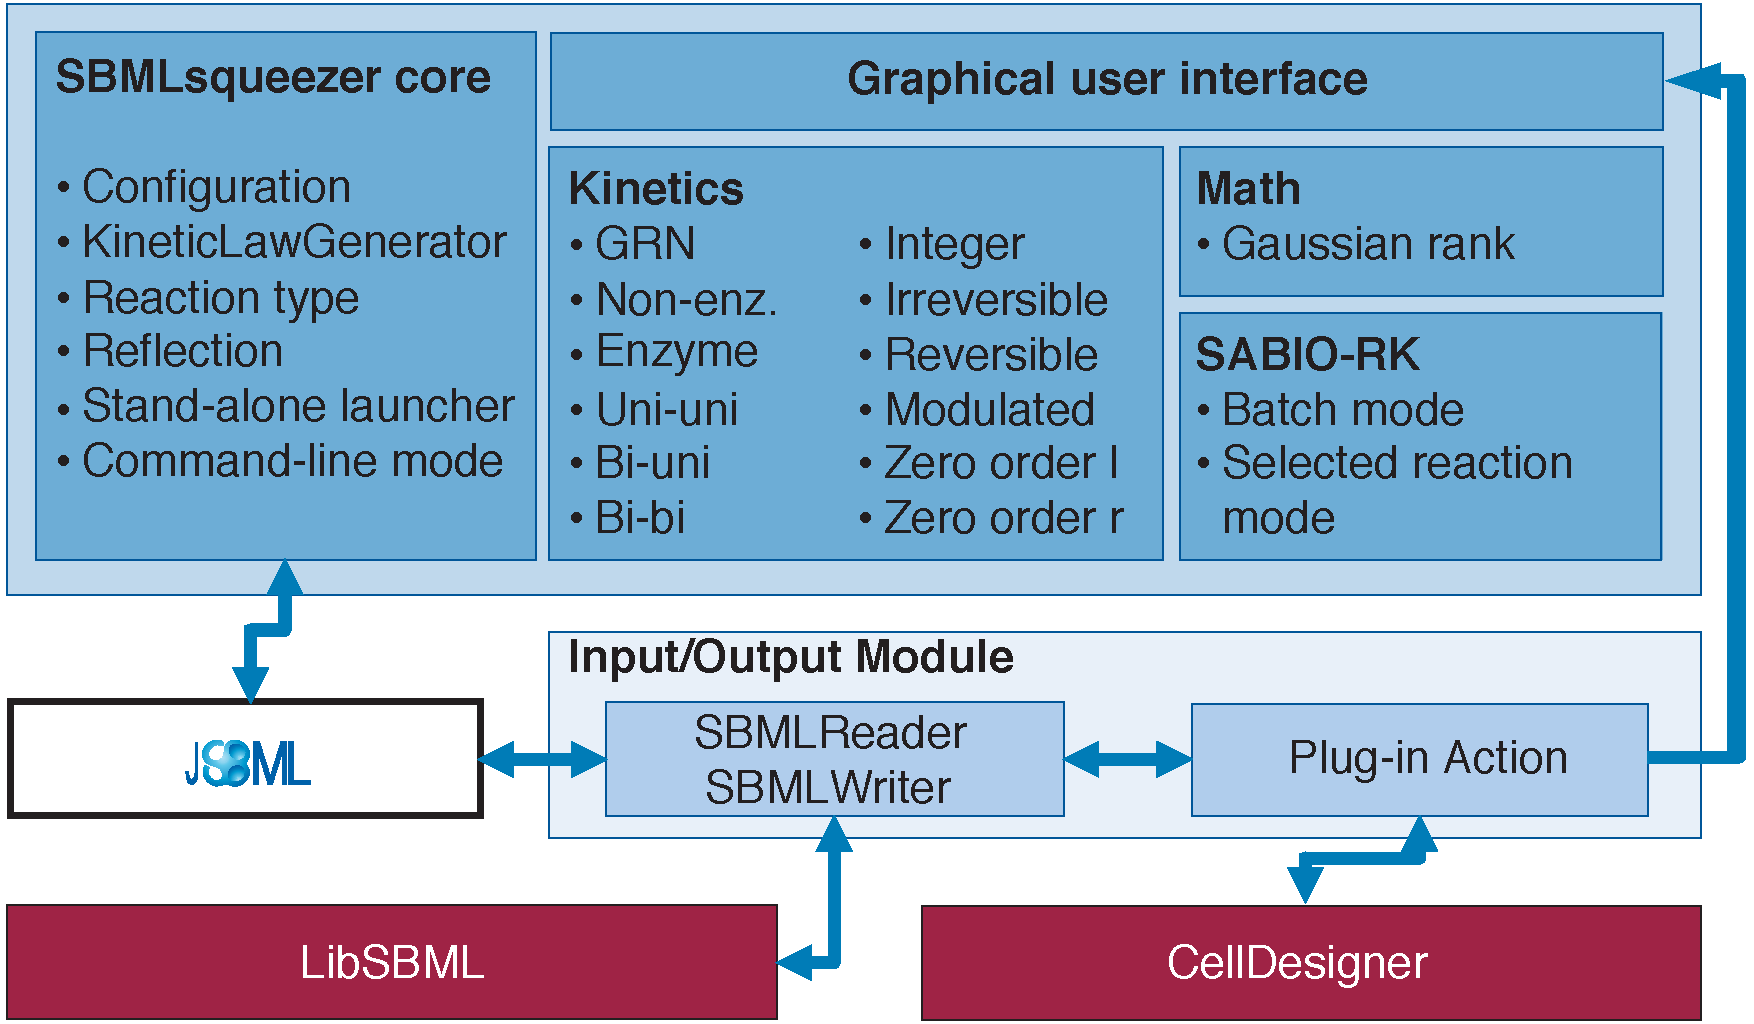
\includegraphics[width=.95\textwidth]{architecture}
  \caption[Architecture of SBMLsqueezer]{Architecture of SBMLsqueezer. The program is organized in several modules that use \JSBML as internal data structure. A compatibility layer enables the program to be used based on \libSBML, \CellDesigner, or as a stand-alone tool (also embedded in \Garuda, an online program etc.). Modified and updated from \citet{Draeger2011a}.}
  \label{fig:architecture}
\end{figure}

SBMLsqueezer consists of a core package that provides a general infrastructure for the program.
The core deals with user preferences and command-line arguments (see \vref{chap:CMD}), and searches for online updates.
Furthermore, the core is responsible to launch the program.
This can be done in diverse ways, e.g., in command line mode, as a plug-in of \CellDesigner, as a gadget in \Garuda etc.

The internal data structure of the program is provided by \JSBML \citep{Draeger2011b}.
Converters can read and write input \SBML documents through \libSBML \citep{Bornstein2008} or \CellDesigner's \API \citep{Funahashi2008}, or \JSBML can directly parse these files.
In this way, \JSBML acts as an abstraction layer between diverse forms of input and synchronizes all changes made by the program back to the original source.
In case that \JSBML is being directly used, the synchronization step can be omitted.

A graphical user interface can be launched from the core and has then control over all functions of the program.
For details about which functions are available and how to use the user interface, see \vref{chap:GUI}.

All implemented rate laws are gathered in the kinetics package and are grouped by twelve interfaces that are described in \vref{sec:RateLawSelection}.
For version~2, a new \SABIO package has been implemented that obtains kinetic equations from the rate law database \SABIO \citep{Wittig2012}.
A mathematics package contains an implementation of the Gaussian rank calculation, which is required for convenience rate laws \citep{Liebermeister2006}.

\section{Rate law selection}
\label{sec:RateLawSelection}

\MIRIAM \citep{Le2005, Laible2007, Juty2012, Juty2013} and \SBO annotations \citep{Courtot2011} constitute the main sources of information for SBMLsqueezer in order to make its choices.
Models can also be evaluated if no such information is given.
However, in these cases the program will most likely make different assignments compared to a fully annotated model.
When used as \CellDesigner plug-in, \SBO terms are inferred from the \CellDesigner-specific annotations of modifiers and further elements.

At first, the algorithm creates a submodel that only comprises those reactions for which rate laws are to be created.
All relevant model components, such as species, compartments, units etc. are copied into this submodel.
Operating on this trimmed copy of the full model has the advantage that changes of the algorithm do not affect the original data structure and can be easily disregarded.
When creating this submodel, the algorithm also checks if fall-back units are defined for all components.
This is crucial in order to avoid problems in later steps.
Depending on which units are missing, it generates units for area, reaction extend, length, substance, time, and volume just as the default units in \SBML Level~2 Version~4 \citep{Hucka2008} would be defined.
All subsequent steps can hence assume that every model component has a defined unit.

The algorithm then iterates trough all reactions within the submodel and performs several pre-processing steps, before an appropriate type of rate law can be selected:
\begin{enumerate}

  \item If the user defines a list of \KEGG \citep{Kanehisa2000a} \acp{ID} for species whose contribution to rate laws should be neglected, species with such terms in their \MIRIAM annotation \citep{Le2005} are removed.
  \Cref{tab:MIRIAMignoreList} shows the predefined list of those entities.
  \item Based on their \SBO term \citep{Courtot2011} attribute all modifiers of the reaction are grouped into the following sets:
  \begin{enumerate*}[label=\itshape\alph*\upshape)]
    \item enzymes;
    \item activators;
    \item inhibitors; and
    \item non-enzyme catalysts.
  \end{enumerate*}
%If the user has decided not to implicitly consider all reactions enzyme-catalyzed, a reaction is considered a \emph{non-enzyme reaction} if either the list of enzymes is empty or there is at least one non-enzyme catalyst, or the reaction is reversible and the set of products is empty.
  Since it is not always clear if a catalyst of a reaction is an enzymatic catalyst, the user can define, which kinds of species may be considered enzymes in the specific context.
  \Cref{tab:EnzymesAndSBO} presents a list of all kinds of species that the algorithm can potentially accept as enzymes of a reaction.
The algorithm checks if any modifier of the reaction corresponds to a species with one of the \SBO terms in this list.
If the modifier is annotated as \emph{catalyst} (\href{http://identifiers.org/biomodels.sbo/SBO:0000013}{\texttt{SBO:0000013}}) and its corresponding species belongs to the list of potential enzymes, the algorithm assigns the \SBO term \emph{enzymatic catalyst} (\href{http://identifiers.org/biomodels.sbo/SBO:0000460}{\texttt{SBO:0000460}}).
Based on the user's selection the algorithm hence solves contradictions between the \SBO term of a modifier and the corresponding species.
\begin{SCtable}[][tb]
\begin{tabular}{ll}
\toprule
Material entity   & \SBO term\\
\midrule
\asRNA            & \href{http://identifiers.org/biomodels.sbo/SBO:0000317}{\texttt{SBO:0000317}}\\
Complex           & \href{http://identifiers.org/biomodels.sbo/SBO:0000253}{\texttt{SBO:0000253}}\\
Generic protein   & \href{http://identifiers.org/biomodels.sbo/SBO:0000252}{\texttt{SBO:0000252}}\\
Macromolecule     & \href{http://identifiers.org/biomodels.sbo/SBO:0000245}{\texttt{SBO:0000245}}\\
Receptor          & \href{http://identifiers.org/biomodels.sbo/SBO:0000244}{\texttt{SBO:0000244}}\\
\RNA              & \href{http://identifiers.org/biomodels.sbo/SBO:0000250}{\texttt{SBO:0000250}}\\
Simple molecule   & \href{http://identifiers.org/biomodels.sbo/SBO:0000247}{\texttt{SBO:0000247}}\\
Truncated protein & \href{http://identifiers.org/biomodels.sbo/SBO:0000248}{\texttt{SBO:0000248}}\\
Unknown molecule  & \href{http://identifiers.org/biomodels.sbo/SBO:0000285}{\texttt{SBO:0000285}}\\
\bottomrule
\end{tabular}
\caption[Kinds of species that can potentially act as enzymes and their top-level \SBO terms]{Kinds of species that can potentially act as enzymes and their top-level \SBO terms.
These \SBO terms correspond to the annotation of the actual species and therefore define the material classes of potential enzymes.
The terms given in this table represent the top-level terms, i.e., the algorithm also accepts each more specialized term for a specific category.
Note that the user can exclude elements from this list and therefore influence the algorithm's choices.}
\protect\label{tab:EnzymesAndSBO}
\end{SCtable}

  \item The stoichiometry of each reaction participant is analyzed in order to obtain the accumulated stoichiometry of reactants and products and to answer the question if all values are integers.
In this step the algorithm analyzes the \SBO term \citep{Courtot2011} attribute of each reaction participant.
Further top-level \SBO terms with relevance to the algorithm can be found in \Cref{tab:FurtherRelevantSBOTerms}.
The aim of this step is to get hints if the reaction represents a transcription or translation:
  \begin{itemize}
    \item If a reactant represents a \gene or gene-coding region, the reaction could be a \transcription.
    \item If the reaction involves a reactant that stands for an \RNA or \mRNA molecule it could be a \translation.
    \item If at least one modifier represents a gene or \RNA molecule, the reaction could represent a \translation.
  \end{itemize}
  \Cref{fig:TranscriptionAndTranslation} depicts these processes in a simple schematic based on the \SBGN recommendations.
  The algorithm recognizes these these reaction patterns only based on the \SBO term annotation of all participants.
%  \begin{SCfigure}
%    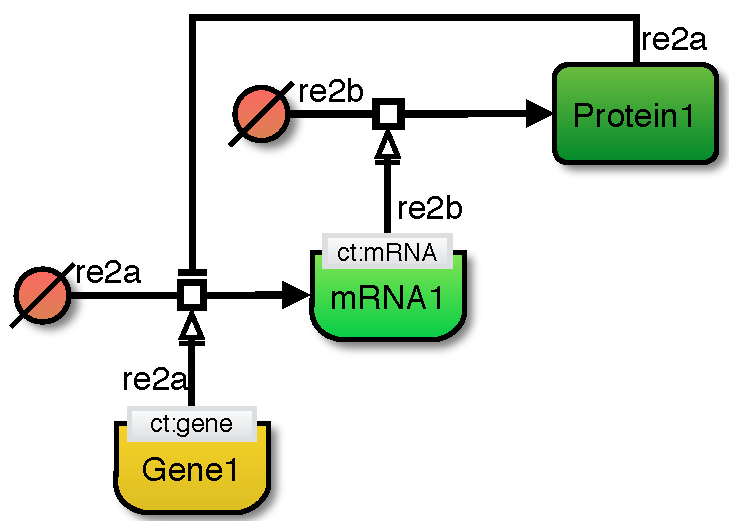
\includegraphics[width=.45\textwidth]{SBGN/GeneRegulatory}
%    \caption[Transcription and translation]{Transcription and translation.
%The first reaction \texttt{re1} assembles an \mRNA molecule from a source of bases.
%The presence of a specific gene enables this process.
%The resulting \mRNA molecule in turn enables the assembly of a protein from a source of amino acids.
%In a feedback inhibition loop, the protein interferes with the transcription of its corresponding gene.}
%    \label{fig:TranscriptionAndTranslation}
%  \end{SCfigure}

  \item In order to ensure that the algorithm can process each reaction within the submodel, it checks the following semantic rules:
  \begin{itemize}
    \item If a reaction involves a \gene or gene-coding region as reactant or its set of reactants is \emph{empty} and all products are \RNA molecules, the reaction is recognized as \transcription.
    \item If the substrate species of a reaction are \RNA molecules or the reaction does not have any reactants and all products are forms of \protein or poly-peptide chains, the reaction is recognized as \translation.
    \item If the stoichiometry of reactants and products is unity, the reaction can only be categorized as \transcription if the only reactant is a \gene or gene-coding region and it is only a valid \translation if the only reactant is an \RNA molecule.
Depending on user preferences, the algorithm can set the boundary condition for each \gene as part of this step.
  \end{itemize}
Note that a list of reactants or products is said to be \emph{empty} if either 
\begin{enumerate*}[label=\itshape\alph*\upshape)]
  \item no such list exists;
  \item no element has been assigned to this list;
  \item the stoichiometry of each element within the list is zero; or
  \item if each element in the list is annotated with an \SBO term derived from the term for \emph{empty set} (\href{http://identifiers.org/biomodels.sbo/SBO:0000291}{\texttt{SBO:0000291}}).
\end{enumerate*}
\end{enumerate}

After having reaction preprocessing and semantic checking completed, the algorithm assigns a list of applicable categories to each reaction within the submodel.
The algorithm distinguishes between the following twelve such categories, which are not necessarily exclusive:\\
\noindent
\begin{minipage}[t]{.5\textwidth}
\raggedleft
\begin{enumerate}
  \item Non-enzyme reactions (\cref{fig:NonEnzymeReactions})
  \item Gene-regulatory processes (\cref{fig:TranscriptionAndTranslation})
  \item Uni-uni enzyme reactions (\cref{fig:UniUniEnzyme})
  \item Bi-uni enzyme reactions (\cref{fig:BiUniEnzyme})
  \item Bi-bi enzyme reactions (\cref{fig:BiBiEnzyme})
  \item Arbitrary enzyme reactions (\cref{fig:ArbitraryEnzyme})
\end{enumerate}
\end{minipage}% <---------------- Note the use of "%"
\begin{minipage}[t]{.5\textwidth}
\raggedleft
\begin{enumerate}
  \setcounter{enumi}{6}
  \item Integer stoichiometry reactions (\cref{fig:IntegerStoichiometry})
  \item Irreversible reactions (\cref{fig:IrreversibleReaction})
  \item Modulated reactions (\cref{fig:ModulatedReaction})
  \item Reversible reactions (\cref{fig:ReversibleReaction})
  \item Zeroth reactant order reactions (\cref{fig:ZerothReactantOrder})
  \item Zeroth product order reactions (\cref{fig:ZerothProductOrder})
\end{enumerate}
\end{minipage}\\[1em]
%\noindent
%\begin{minipage}[t]{.5\textwidth}
%\raggedleft
%\begin{enumerate}
%  \item gene-regulatory and transcriptional reactions,
%  \item zeroth reactant order reactions,
%  \item zeroth product order reactions,
%  \item reversible reactions with an optional non-enzyme catalyst,
%  \item irreversible reactions with an optional non-enzyme catalyst,
%  \item reversible enzyme-catalyzed reactions with an arbitrary number of reactants or products,
%  \item irreversible enzyme-catalyzed reactions with an arbitrary number of reactants or products,
%\end{enumerate}
%\end{minipage}% <---------------- Note the use of "%"
%\begin{minipage}[t]{.5\textwidth}
%\raggedleft
%\begin{enumerate}
%  \setcounter{enumi}{7}
%  \item reversible uni-uni type enzyme-catalyzed reactions,
%  \item irreversible uni-uni type enzyme-catalyzed reactions,
%  \item reversible bi-uni type enzyme-catalyzed reactions,
%  \item irreversible bi-uni type enzyme-catalyzed reactions,
%  \item reversible bi-bi type enzyme-catalyzed reactions, and
%  \item irreversible bi-bi type enzyme-catalyzed reactions.
%\end{enumerate}
%\end{minipage}\\[1em]
%\begin{enumerate}
%  \item gene-regulatory reactions,
%  \item zeroth reactant/product order reactions,
%  \item reversible/irreversible reactions with an optional non-enzyme catalyst,
%  \item reversible/irreversible enzyme-catalyzed reactions with an arbitrary number of reactants or products,
%  \item reversible/irreversible uni-uni type enzyme-catalyzed reactions,
%  \item reversible/irreversible bi-uni type enzyme-catalyzed reactions, and
%  \item reversible/irreversible bi-bi type enzyme-catalyzed reactions.
%\end{enumerate}
\begin{figure}[htbp]
  \centerline{
    \subfloat[A non-enzyme reaction. The ion ``I1'' catalyzes this association reaction, which can therefore not be considered enzyme catalyzed. In addition, this reaction is also modulated in a feedback inhibition loop, has an integer stoichiometry, and two reactants.]{\label{fig:NonEnzymeReactions}%
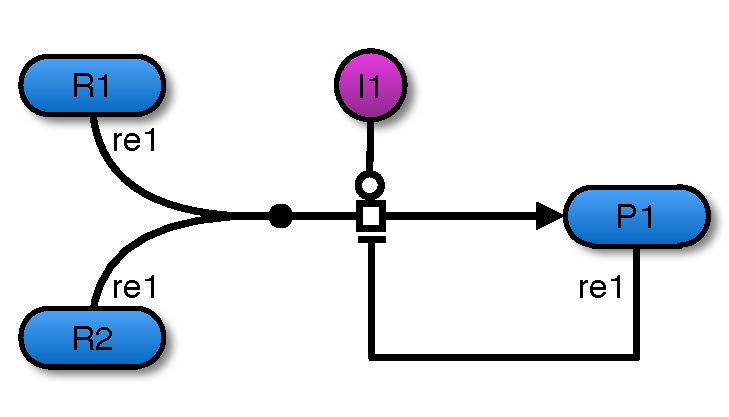
\includegraphics[width=.45\textwidth]{SBGN/IrreversibleNonEnzyme}}\hfill%
   \subfloat[Gene-regulatory processes.
Reaction \texttt{re2a} assembles an \ac{mRNA} molecule from a source of bases (transcription), enabled by the a specific gene.
This \ac{mRNA} in turn (\texttt{re2b}) enables the assembly of a protein from a source of amino acids (translation).
In a feedback inhibition loop, the protein interferes with the transcription of its own gene.]{\label{fig:TranscriptionAndTranslation}%
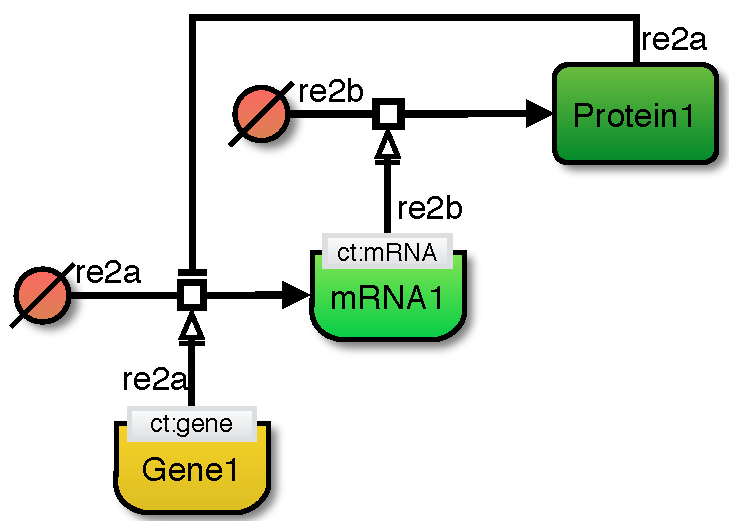
\includegraphics[width=.45\textwidth]{SBGN/GeneRegulatory}}}
  \centerline{\subfloat[Uni-uni enzyme reaction. This schematic conforms the classical Michaelis-Menten mechanism.]{\label{fig:UniUniEnzyme}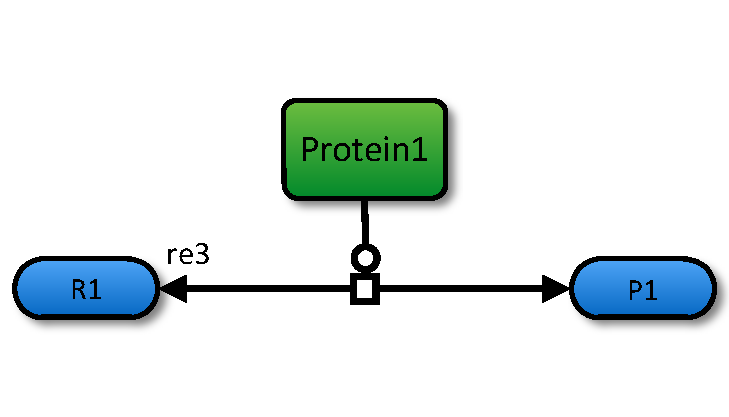
\includegraphics[width=.45\textwidth]{SBGN/ReversibleUniUniEnzyme}}\hfill\subfloat[Bi-uni enzyme reaction. This association reaction has an integer stoichiometry.]{\label{fig:BiUniEnzyme}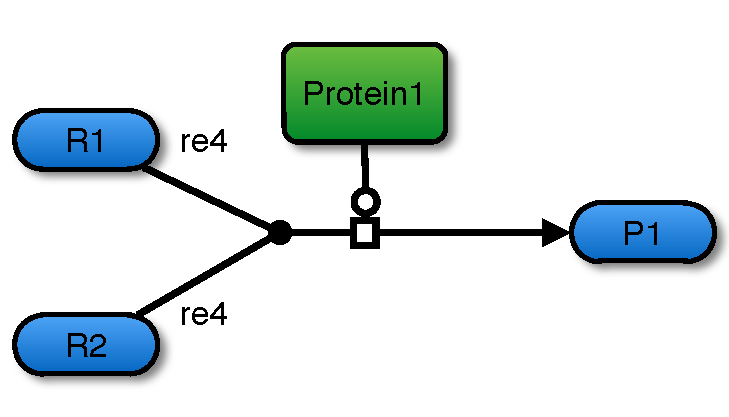
\includegraphics[width=.45\textwidth]{SBGN/IreversibleBiUniEnzyme}}}
  \centerline{\subfloat[Bi-bi enzyme reaction. In this example, two molecules of identical type act as reactants and also as products, respectively.]{\label{fig:BiBiEnzyme}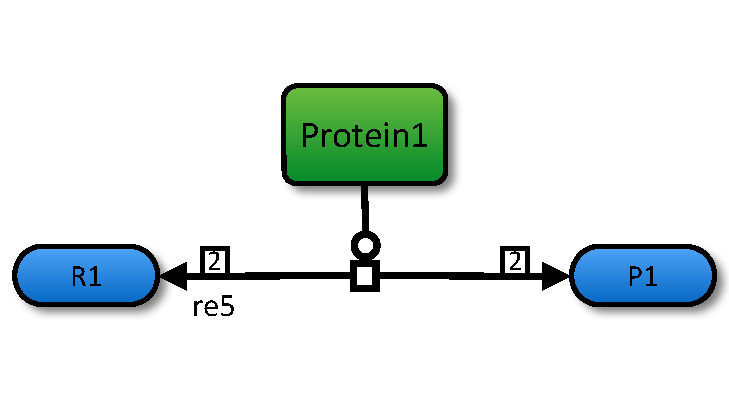
\includegraphics[width=.45\textwidth]{SBGN/IrreversibleBiBiEnzyme}}\hfill\subfloat[Arbitrary enzyme reaction. This reversible reaction involves a feedback inhibition and a complex stoichiometry, in which an ion and two identical molecules are created from two distinct reactants.]{\label{fig:ArbitraryEnzyme}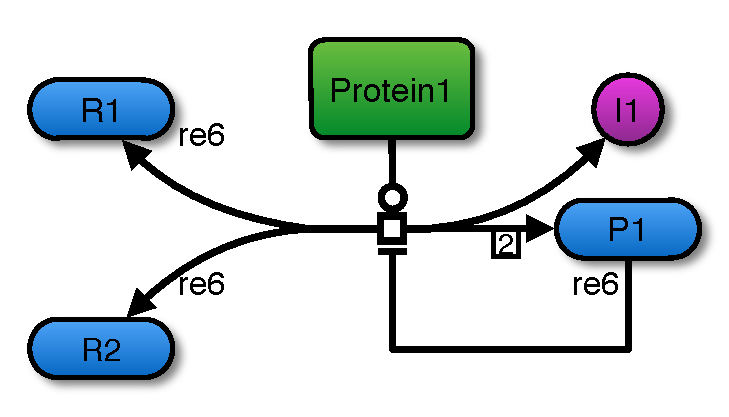
\includegraphics[width=.45\textwidth]{SBGN/ReversibleArbitraryEnzyme}}}
  \caption[Examples for general reaction categories]{Examples for general reaction categories. This figure displays example reactions in \SBGN for each of the twelve categories that are used to determine applicable rate equations.}\label{fig:ReactionCategories}%
\end{figure}
\begin{figure}[htbp]
  \ContinuedFloat
  \centerline{\subfloat[Integer stoichiometry. This reversible, enzyme-catalyzed reaction has two identical reactants and one product.]{\label{fig:IntegerStoichiometry}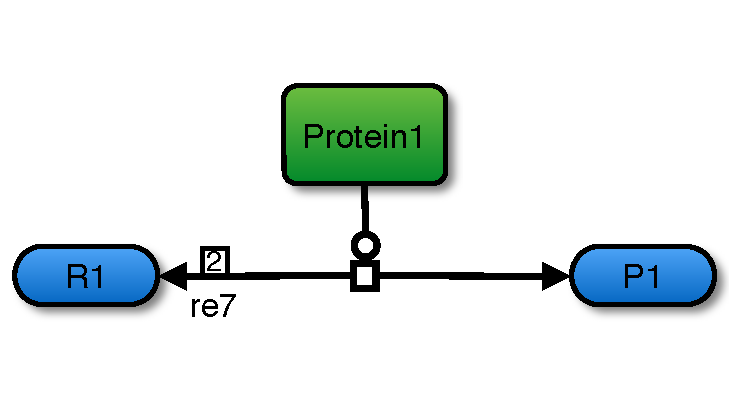
\includegraphics[width=.45\textwidth]{SBGN/ReversibleBiUniEnzyme}}\hfill\subfloat[Irreversible reaction. This reaction has no explicit catalyst assigned to it. Depending on user-settings, the algorithm can still consider this an enzyme-catalyzed reaction, assuming that the omission of the catalyst is for the sake of simplicity.]{\label{fig:IrreversibleReaction}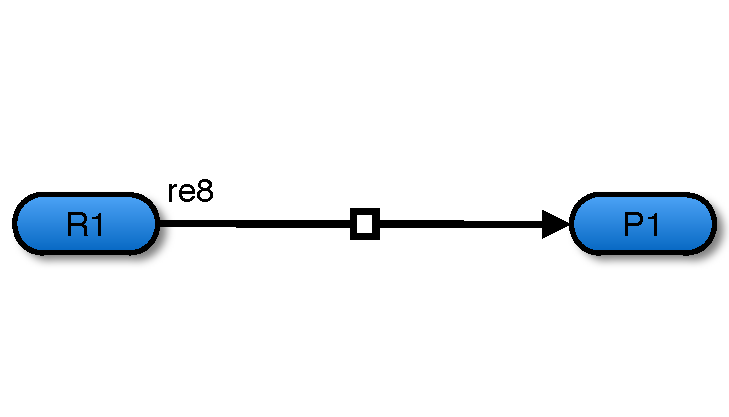
\includegraphics[width=.45\textwidth]{SBGN/IrreversibleUniUni}}}
  \centerline{\subfloat[Modulated reaction. Both, a stimulator and an inhibitor interfere with this reaction.]{\label{fig:ModulatedReaction}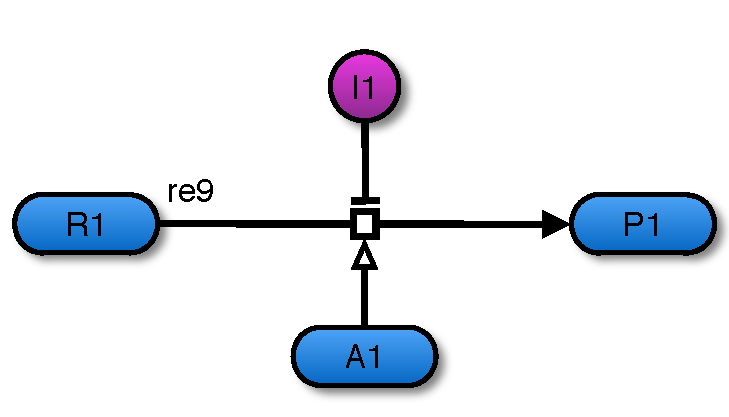
\includegraphics[width=.45\textwidth]{SBGN/IrreversibleUniUniModulated}}\hfill\subfloat[Reversible reaction. This dissociation reaction can also be seen as an association when the equilibrium shifts to the reverse reaction.]{\label{fig:ReversibleReaction}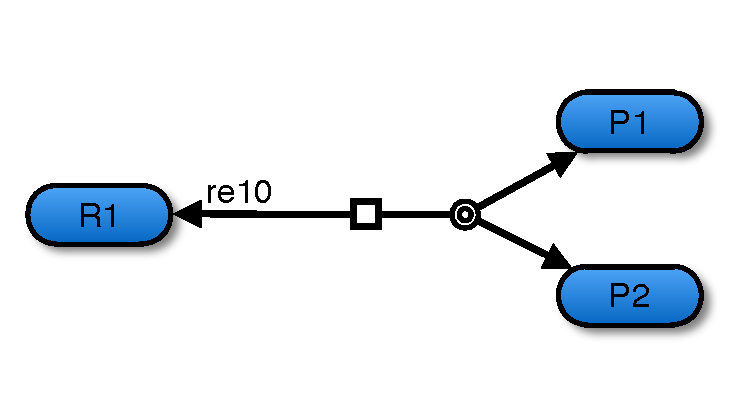
\includegraphics[width=.45\textwidth]{SBGN/ReversibleReaction}}}
  \centerline{\subfloat[Zeroth reactant order reaction. The two product molecule lower the velocity of their own creation.]{\label{fig:ZerothReactantOrder}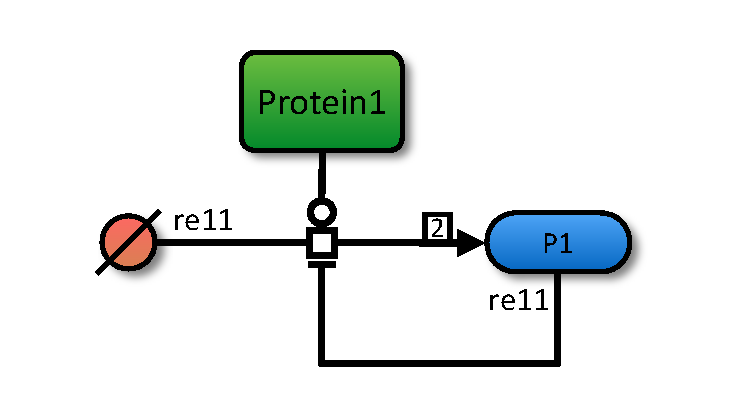
\includegraphics[width=.45\textwidth]{SBGN/ZerothOrderReactants}}\hfill\subfloat[Zeroth product order reaction. The reactant stimulates its own degradation.]{\label{fig:ZerothProductOrder}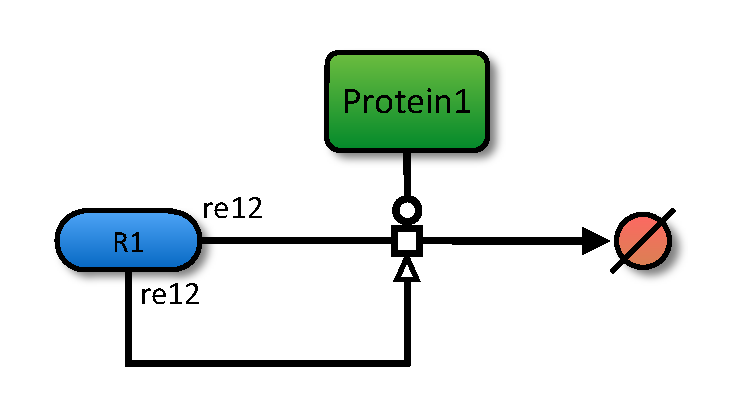
\includegraphics[width=.45\textwidth]{SBGN/ZerothOrderProducts}}}
  \caption[Examples for general reaction categories (continued)]{Examples for general reaction categories (continued)}\label{fig:Continued}
\end{figure}

All kinetic equations are also assigned to one or multiple of these categories.
The algorithm may now either collect all appropriate rate laws for the obtained reaction categories (types) or just the one rate law with highest priority.
While the first method allows users to interactively select rate laws of choice, the latter option is important for the automatic selection of the most appropriate equation.
\begin{SCtable}
\begin{tabular}{ll}
\toprule
Definition & \SBO term\\
\midrule
catalyst                   & \href{http://identifiers.org/biomodels.sbo/SBO:0000013}{\texttt{SBO:0000013}}\\
empty set                  & \href{http://identifiers.org/biomodels.sbo/SBO:0000291}{\texttt{SBO:0000291}}\\
enzymatic catalyst         & \href{http://identifiers.org/biomodels.sbo/SBO:0000460}{\texttt{SBO:0000460}}\\
gene                       & \href{http://identifiers.org/biomodels.sbo/SBO:0000243}{\texttt{SBO:0000243}}\\
gene-coding region         & \href{http://identifiers.org/biomodels.sbo/SBO:0000335}{\texttt{SBO:0000335}}\\
generic                    & \href{http://identifiers.org/biomodels.sbo/SBO:0000252}{\texttt{SBO:0000252}}\\
inhibition                 & \href{http://identifiers.org/biomodels.sbo/SBO:0000169}{\texttt{SBO:0000169}}\\
inhibitor                  & \href{http://identifiers.org/biomodels.sbo/SBO:0000020}{\texttt{SBO:0000020}}\\
\mRNA                      & \href{http://identifiers.org/biomodels.sbo/SBO:0000278}{\texttt{SBO:0000278}}\\
necessary stimulation      & \href{http://identifiers.org/biomodels.sbo/SBO:0000171}{\texttt{SBO:0000171}}\\
protein                    & \href{http://identifiers.org/biomodels.sbo/SBO:0000297}{\texttt{SBO:0000297}}\\
\RNA                       & \href{http://identifiers.org/biomodels.sbo/SBO:0000250}{\texttt{SBO:0000250}}\\
stimulation                & \href{http://identifiers.org/biomodels.sbo/SBO:0000170}{\texttt{SBO:0000170}}\\
stimulator                 & \href{http://identifiers.org/biomodels.sbo/SBO:0000021}{\texttt{SBO:0000021}}\\
transcriptional activation & \href{http://identifiers.org/biomodels.sbo/SBO:0000459}{\texttt{SBO:0000459}}\\
transcriptional inhibition & \href{http://identifiers.org/biomodels.sbo/SBO:0000020}{\texttt{SBO:0000020}}\\
translational activation   & \href{http://identifiers.org/biomodels.sbo/SBO:0000459}{\texttt{SBO:0000459}}\\
trigger                    & \href{http://identifiers.org/biomodels.sbo/SBO:0000461}{\texttt{SBO:0000461}}\\
translation                & \href{http://identifiers.org/biomodels.sbo/SBO:0000184}{\texttt{SBO:0000184}}\\
transcription              & \href{http://identifiers.org/biomodels.sbo/SBO:0000183}{\texttt{SBO:0000183}}\\
\bottomrule
\end{tabular}
\caption[\SBO terms with relevance for the categorization of reactions]{\SBO terms with relevance for the categorization of reactions.
The algorithm uses the \SBO terms listed in this table in order to distinguish between different types of species and modification in order to categorize a each reaction in the submodel as well as the role of individual reaction participants.
This also includes further relevant material entities of reaction participants.
Note that the algorithm always checks if the \SBO term of an element is a child of a certain reference term in order to also include all more specific sub-terms.}
\label{tab:FurtherRelevantSBOTerms}
\end{SCtable}
%
The selection of one or multiple appropriate categories and in turn suitable kinetic equations for a reaction is based on a set of defined rules, which are here summarized and simplified for the sake of better comprehensiveness.
%
The algorithm distinguishes the following three basic cases, which are not necessarily exclusive:
\begin{enumerate}
  \item The list of reactants is \emph{empty} or the reaction is reversible and the list of products is \emph{empty}.
If the reaction does neither involve genes, gene-coding regions, nor \RNA molecules, then the algorithm can assign it to the  zeroth reactant order reactions if also the list of reactants is \emph{empty}, and to the zeroth product order reactions if it is reversible with an empty list of products.
If it does involve genetic components, it can be assigned to the gene-regulatory reactions depending on its directionality.

  \item The reaction has at least one reactant and if it is reversible also at least one product.
If the reaction does neither have any enzymatic catalyst nor any non-enzymatic catalyst, it is assigned to the category of non-enzyme reactions with respect to its directionality.
In case of unity stoichiometry on both sides of the reaction, and if the reaction follows the pattern of \transcription or \translation reactions, it is added to the category of gene-regulatory reactions.
The pattern is satisfied if the reactant is a genetic element or an empty set and the product is an \RNA molecule or \protein.

  \item The preprocessing has revealed that the reaction belongs to enzyme kinetics.
Depending on user preferences, a reaction can also be recognized as enzyme-catalyzed process if no catalytic modifier is assigned to it.
If the reaction is reversible with at least one product, the category of arbitrary enzyme reactions is assigned.
Next, the stoichiometry and directionality of the reaction are taken into account in order to determine if the reaction also belongs to the uni-uni, bi-uni, or bi-bi reactions.
\end{enumerate}
The identification of the category with highest priority works very similar.
For reactions with empty list of reactants a gene-regulatory reaction has higher priority than the zeroth reactant order (but requires that the reaction follows the right pattern).
Similarly, the algorithm first tries to assign a reaction to the gene-regulation category if it is reversible with an empty list of products, before assigning it to the zeroth product order reactions.
Non-enzymatic reactions have higher priority than any enzymatic reaction.
If the reaction is enzyme-catalyzed, the algorithm tries to first assign the most detailed category before it chooses an arbitrary enzyme reaction category.

Each reaction category is represented with one interface that can be implemented by rate laws that are applicable for this category.
Since one rate law can be useful for multiple categories, rate laws can also implement several of these interfaces.
For all categories that can be applied to a reaction, the algorithm then compiles a list of concrete kinetic equations using a concept known as \emph{reflection}.
%One post-processing step is required to modify the list of assignable rate laws.
%Not each equation can be applied to reactions that are modulated by activators or inhibitors.
%In this situation, inappropriate equations are subsequently removed from the list of equations.
%The group of those kinetic equations also implements a common interface and can therefore also be identified on run-time.
The list of applicable kinetic equations is hence generated on the fly and only based on the general reaction categories.
In this way, the program can easily be extended, because additional kinetic equations only need to declare the categories to which they can be applied and will automatically be available when the program is executed.

Additional rules apply when the algorithm compiles the list of rate laws based on reaction categories, because some rate laws can only be applied to certain combinations of categories.
For instance, the \emph{enzymatic rate law for irreversible non-modulated non-interacting uni-reactant enzymes} (\href{http://identifiers.org/biomodels.sbo/SBO:0000150}{\texttt{SBO:0000150}}) can only be applied to irreversible reactions with integer but arbitrary stoichiometry, but does not allow stimulators or inhibitors.
Thus, some categories exclude certain rate laws from being assigned to a reaction.

The user can select one default rate law for almost all categories.
No specific default rate law can be selected for the categories irreversible or reversible reactions, modulated reactions, or integer stoichiometry, because these cases mainly refine the other categories.
Instead, the selection of default rate laws is split into three major groups:
\begin{enumerate*}[label=\itshape\alph*\upshape)]
  \item gene-regulatory reactions (including reactions with zeroth order reactants or products);
  \item reversible reactions; and
  \item irreversible reactions.
\end{enumerate*}
This is necessary because some rate laws can only be applied to reversible reactions, others only to irreversible reactions.
If one kinetic equation is to be created for all reactions in a given model, the algorithm determines one category for each reaction and applies the default rate law from this category to the reaction.
In case of conflicts there are two final fall-back rate laws that can be applied if not other rate law can be selected:
\begin{enumerate*}[label=\itshape\alph*\upshape)]
  \item for non-enzyme reactions, the generalized mass-action rate law \citep{Guldberg1879, Heinrich1996}; and
  \item the convenience rate law \citep{Liebermeister2006} for any kind of enzyme-catalyzed reaction.
\end{enumerate*}
Both rate laws can be applied to reversible and irreversible reactions with arbitrary stoichiometry and can be combined with pre-factors for modification (activation or inhibition) as needed.
When creating rate laws for individual reactions, a complete list of all applicable rate laws for the reaction of interest is compiled.

When convenience rate laws are used, the algorithm prefers the simple form and applies the thermodynamically independent form only if the system does not have full column rank. To this end, the program calculates the rank of the stoichiometric matrix using the Gaussian algorithm. This rank check is performed only once for the given submodel and only executed if at least one reaction exists, for which a convenience rate law is selected.

Applying a rate law to the reaction means that the algorithm has to construct an abstract syntax tree, which symbolically represents the kinetic equation for the reaction.
To this end, the reaction needs to be analyzed again and all of its components need to be taken into account as relevant for the selected rate law (irreversible equations, for instance, tend to ignore effects of products).
An example for such an syntax tree can be seen in \vref{fig:AST}, which has been created for the reaction schematic displayed in \vref{fig:IrreversibleReaction}.
\begin{SCfigure}
  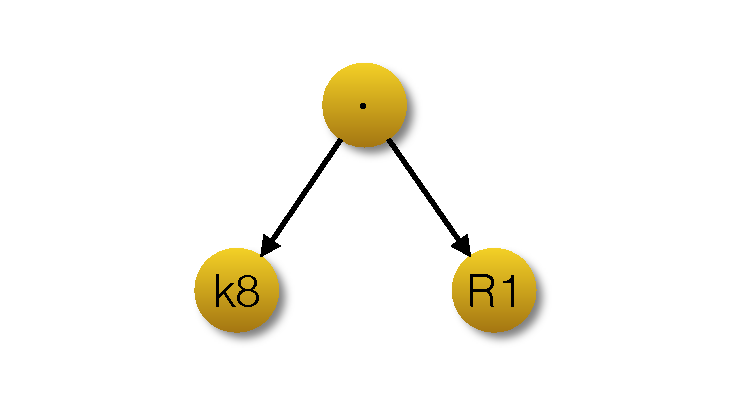
\includegraphics[width=.45\textwidth]{SBGN/AST}
  \caption[Abstract syntax tree for an irreversible mass-action rate law]{Abstract syntax tree for an irreversible mass-action rate law. This tree represents the rate law $\nu_8 = k_8\cdot [R_1]$. The program internally constructs all equations in form of syntax trees, which can contain references to objects in the \ac{SBML} document.}
  \label{fig:AST}
\end{SCfigure}

In order to ensure unit consistency of the equation, it can be necessary to multiply or divide reactive species with/by their surrounding compartment.
User preferences and the units of the species determine if and which of those operation is required, because in \SBML, each reaction should yield units of extent per time.
Two cases need to be distinguished:
\begin{enumerate}
  \item If a species has only substance units and the user decides to bring all species to concentration units, the species must be divided by its surrounding compartment.
  \item If a species is given in concentration units and the user wants to bring all species to substance units, then a multiplication of the species with its surrounding compartment is required.
\end{enumerate}

Depending on the type of rate law that is being created and the structural composition of the reaction, a certain number of parameters needs to be constructed.
This can include forward or backward rate constants, limiting velocity rates, inhibition or stimulation constants, thermodynamic properties, and many more.
These parameters can be incorporated as local or global parameters.
To this end, the algorithm first collects all parameters in a separate list and transfers them to the submodel only when a rate law is to be applied.
Just as for species, parameter objects need to be equipped with appropriate units.
The units of many parameters also depend on the structure of the reaction, for instance, the number and units of all reactants.
Because of this connection, it can be necessary to also take the units of compartments into account when deriving the units of parameters in order to obtain extend by time units for the overall rate law.
The algorithm equips each newly created parameter with a meaningful name and identifier as well as an appropriate \SBO term.
If during this step additional units or unit definitions need to be added to the submodel, these are simplified as much as possible, annotated with a \MIRIAM identifier pointing to the Units Ontology, and equipped with meaningful names and identifiers as appropriate.
The algorithm avoids creating duplicate unit definitions by checking the model for identical existing unit definitions before adding a new one.
If possible, the newly created kinetic equation is also annotated with a corresponding \SBO term.
Due to the large number of \SBO terms that can be created by the algorithm, a comprehensive list of all cases is omitted in this document.

Whenever a kinetic equation that involves stoichiometry values is created for models in \SBML Level~3, the algorithm inserts the \ID of the corresponding species reference rather than the actual numerical value of the stoichiometry into the rate law.
This gives the advantage that model changes can be directly reflected in the rate law, hence increasing the consistency of models.
At the same time, it avoids the problem that units and meaning of single numerical values might not always be clear.

Finally, all relevant changes in the submodel are synchronized to the original model.
This includes all newly created units and unit definitions, local and global parameters, annotations, mathematical equations, reversibility flags, and boundary condition flags.
If species have been deleted from reactions, because their \MIRIAM annotation was on the ignore list, this change is skipped and not synchronized, so that the structure of the model will remain identical.
In the graphical user interface, the user can also disregard the changes.
When being used as a \CellDesigner plug-in, a special observer class synchronizes all changes from the submodel to the data model of \CellDesigner.

\section{Extraction of rate laws from \SABIO}

The extraction of rate laws from the database \SABIO requires an \SBML document and search terms as input.
All possible values for the search terms can be found in \vref{sec:SABIO_search_options}.

The algorithm first generates a \URL that is used to query the \SABIO database.
This \URL comprises the search terms and the respective \KEGG reaction \ac{ID}.
The \URL begins with the prefix \url{http://sabio.h-its.org/sabioRestWebServices/searchKineticLaws/sbml?q=}.
Each search term and its given value extend this base \URL with \texttt{keyword:value}.
If a search term is associated with a range (e.g., the temperature), the \URL is extended with \texttt{keyword:[min\textvisiblespace{}TO\textvisiblespace{}max]}.
The keywords for the terms are presented here: \url{http://sabio.h-its.org/layouts/content/docuRESTfulWeb/SearchKeyVoc.gsp}.
The operator \texttt{\textvisiblespace{}AND\textvisiblespace} connects multiple keyword-value pairs in the query.

The \URL for querying points to an \XML document for download.
In the case of success, the \XML document will be an \SBML document with all kinetic laws found for the query.
Otherwise, \SABIO returns an \XML document with an error message and the algorithm terminates with a user message.

Just like for the \emph{de novo} creation of rate laws the algorithm can either process all reactions within the \SBML document or one particular reaction.
To this end, the algorithm creates one query \URL for each reaction, for which a rate law should be extracted from \SABIO.
After obtaining an \SBML document from \SABIO, the algorithm extracts all kinetic laws from the \SBML document and tries to match all elements contained in a kinetic law to elements in the input network. 
This matching is based on the \MIRIAM annotations of model components and involves the search for one corresponding
\begin{itemize}
  \item species in the local model for each species that participates in the kinetic law.
  \item compartment in the local model for each compartment addressed in the kinetic law (this can be the compartment of a participating species or the reaction itself can have a compartment assigned to it).
  \item reaction in the local model for each reaction in the kinetic law.
  \item species reference for each species reference in the kinetic law within each such identified local reaction. 
This species reference needs to refer to a species with an annotation similar to that of the species referenced by the species reference in the found rate law.
\end{itemize}
In this context, an annotation of two \SBML elements is considered similar and hence these elements are considered a \emph{match} if both have \emph{controlled vocabulary terms} in common that are linked through qualifiers \emph{has version} or \emph{is}.

In the batch mode, the algorithm always selects the first kinetic law in the query results for which all elements can be matched to respective elements in the model.
The algorithm adds this rate law to the reaction.
This merging involves
\begin{enumerate}
  \item Substituting all elements in the found kinetic law with the matched elements in the model.
  \item Adding unit definitions, function definitions, global and local parameters contained in the kinetic law to the model.
\end{enumerate}

Since this algorithm mainly operates on models obtained from \SABIO it is not necessary to create a submodel copy of the local model beforehand (as this is done for the \emph{de novo} creation of rate laws).
Changes are only applied upon user agreement or in batch mode.
This is done by merging required components from the downloaded model into the local model.
For this reason, the local model does not change, before rate laws are applied.

When rate laws are obtained from \SABIO for individual reactions, the algorithm presents a list of all rate laws found for the given query to the user, who can then select the most appropriate equation.
In cases when the selection of the first law with a successful matching does not lead to a satisfying result, the single reaction mode might yield better results.


% 03_Troubleshooting
\chapter{\acs{FAQ} and troubleshooting}
\label{ch:faq}

%\TODO{These are some template questions. Add new ones and modify/ remove the old ones to suit your needs.}

\noindent \textbf{Where can I get help for a certain component, option, check-box etc.?}\newline
Most elements in SBMLsqueezer have tool-tips. If you do not understand an option, you
can get help in the first place by just pointing the mouse cursor over it and
wait for the tool-tip to show up ($\sim$3 seconds).\newline

\noindent \textbf{I'm getting a ``java.lang.OutOfMemoryError: Java heap space"}\newline
Some operations need a lot of memory. If you simply start SBMLsqueezer, without any
\JVM parameters, only 64\,MB of memory are available. Please append the argument
\texttt{-Xmx1024M} to start the application with 1\,GB of main memory. See
\vref{sec:Program_usage} for a more detailed description of how to
start the application with additional memory. If possible, you should give the
application 2\,GB of main memory. A minimum of 1\,GB main memory should be
available to the application.\newline

\noindent \textbf{Is an Internet connection required to run SBMLsqueezer?}\newline
The vast majority of SBMLsqueezer's functions run in off-line mode.
Features that require an active Internet connection are the online check for updates, the extraction of rate laws from the online database \SABIO, and following external links within online help.
\newline

\noindent \textbf{Where can I obtain the latest version?}\newline
Go to \url{http://www.cogsys.cs.uni-tuebingen.de/software/SBMLsqueezer/}.\newline

\noindent \textbf{Which \Java version must be installed on my computer to launch SBMLsqueezer?}\newline
SBMLsqueezer requires at least \Java 1.6. Please see \url{http://www.java.com/de/download/} to download the latest \Java version.\newline

\noindent \textbf{Why does SBMLsqueezer not start on my Mac with \MacOSX prior to 10.6 Update 3?}\newline
If you try to launch SBMLsqueezer, but the application does not start and you receive the following error message on the command-line or \Java console of your Mac, you need to update your \Java installation:
\begin{verbatim}
Exception in thread "AWT-EventQueue-0" java.lang.NoClassDefFoundError:
    com/apple/eawt/AboutHandler
    at java.lang.ClassLoader.defineClass1(Native Method)
    at java.lang.ClassLoader.defineClass(ClassLoader.java:703)
    ...
\end{verbatim}
The interface \texttt{com.apple.eawt.AboutHandler} was introduced to \Java for \MacOSX 10.6 Update 3. If you have an earlier version of \MacOSX or \Java, please update your OS or \Java installation.
Also see the \MacOSX documentation about the \texttt{AboutHandler} for more information. On a Mac, you can update your \Java installation through the Software Update menu item in the main Apple menu.
\newline

\noindent \textbf{How can I report bugs or get help?}\newline
Please contact the mailing list using the e-mail address \ding{41}
\href{mailto:sbmlsqueezer@googlegroups.com}{\texttt{sbmlsqueezer@google\-groups.com}}.

\chapter{License}

\section{Disclaimer}
\begin{wrapfigure}{O}{1.5cm}
\vspace{\wrapfigspace}

\includegraphics[width=1.5cm]{lgplv3-147x51}
\end{wrapfigure}
SBMLsqueezer is free software: you can redistribute it and/or modify
it under the terms of the \acf{GPL} as published by
the Free Software Foundation, either version~3 of the License, or
(at your option) any later version.

This program is distributed in the hope that it will be useful,
but \textbf{without any warranty}; without even the implied warranty of
\textbf{merchantability} or \textbf{fitness for a particular purpose}. See the
GNU General Public License for more details.

Each distributed version of SBMLsqueezer should contain a copy of the 
GNU General Public License. If not, please see
\href{http://www.gnu.org/licenses/gpl-3.0-standalone.html}{\nolinkurl{http://www.gnu.org/licenses/}}.


\section{Included third-party libraries}
SBMLsqueezer includes and re-distributes the following third-party software libraries.
\begin{itemize}
  \item \JSBML (1.0$\beta$1, revision 1697) including all of its third-party libraries, see \url{http://sbml.org/Software/JSBML}.
  \item \JUnit (version 4.8, Eclipse Public License), see \url{http://junit.org/}.
  \item \SBMLLaTeX (build 20140410-1447, \GPL), see \url{http://sourceforge.net/projects/sbml2latex/} and \url{http://www.cogsys.cs.uni-tuebingen.de/software/SBML2LaTeX/}.
  \item \libSBML (version 5.9.0, \LGPL), see \url{http://sbml.org/Software/libSBML}.
  \item Quaqua filechooser (version 9, \LGPL), see \url{http://www.randelshofer.ch/quaqua/}.
  \item \Garuda (version 1.0$\beta$1) including all of its third-party libraries, see \url{http://www.garuda-alliance.org}.
  \item jlatexmath (version 1.0.0, \GPL), see \url{http://forge.scilab.org/index.php/p/jlatexmath/}.
\end{itemize}
All version numbers are given with respect to the latest release of SBMLsqueezer.

\chapter{Acknowledgments}

This work has been funded by a Marie Curie International Outgoing Fellowship
awarded to Andreas Dr\"ager within the EU 7\textsuperscript{th} Framework
Program for Research and Technological Development (project AMBiCon, 332020) and
by the Federal Ministry of Education and Research (BMBF, Germany) in the
projects Virtual Liver Network (project number 0315756), National Genome
Research Network (NGFN-Plus, project number 01GS08134), and Spher4Sys (grant
number 0315384C).

\section{Core developers}

The following people implemented wide parts of SBMLsqueezer:
\begin{itemize}
\item Andreas Dr\"ager, 
  University of California, San Diego, La Jolla, California, USA and
  University of Tuebingen, Germany
  \href{mailto:andraeger@eng.ucsd.edu}{andraeger@eng.ucsd.edu}
\item Roland Keller,
  University of Tuebingen, Germany
  \href{mailto:roland.keller@uni-tuebingen.de}{roland.keller@uni-tuebingen.de}
\item Johannes Eichner,
  University of Tuebingen, Germany
  \href{mailto:johannes.eichner@uni-tuebingen.de}{johannes.eichner@uni-tuebingen.de}
\end{itemize}

\section{Principal Investigators}

\begin{itemize}
\item Bernhard \O.~Palsson,
  University of California, San Diego, La Jolla, California, USA
  \href{mailto:palsson@ucsd.edu}{palsson@ucsd.edu}
\item Andreas Zell, 
  University of Tuebingen, Germany
  \href{mailto:andreas.zell@uni-tuebingen.de}{andreas.zell@uni-tuebingen.de}
\end{itemize}

\section{Alumni}

During the years, many people contributed to this project.
We are grateful to each contribution, such as source code, advice, proof reading
and much more. In particular, we like to thank our former scientific advisors,
colleagues, and students, who are here listed all together in alphabetical
order:
Meike Aichele,
Hannes Borch,
Alexander D\"orr,
Nadine Hassis,
Marcel Kronfeld,
Oliver Kohlbacher,
Sarah Rachel M\"uller vom Hagen,
Sebastian Nagel,
Leif J.~Pallesen,
Alexander Peltzer,
Julianus Pfeuffer,
Sandra Saliger,
Simon Sch\"afer,
Adrian Schr\"oder,
Jochen Supper,
Dieudonn\'e M.~Wouamba,
Michael J.~Ziller

We also thank Shaowu Yang for providing the \Chinese language pack for this program.


\section{Collaborators and partners}

The authors are grateful to the \SABIO team, in particular Martin Golebiewski and Wolfgang M\"uller from the Heidelberg Institute of Technology (HITS).

%\section{Disclaimer}
%
%This document does not claim affiliation or endorsement of any of the authors with any of the producers of commercial software products that are mentioned throughout this text.
%In particular, none of the authors is affiliated with Apple, Microsoft, Oracle, neither involved in the development, implementation, or distribution of their commercial software products, such as \Java, \Windows, \MacOSX.




%%%%%%%%%%%%%%%%%%%%%%%%%%%%%%%%%
% Das Literaturverzeichnis      %
%%%%%%%%%%%%%%%%%%%%%%%%%%%%%%%%%

\bibliographystyle{natbib}
\bibliography{tex/literature}

\end{document}
